\documentclass[final]{beamer}

% =====================================================================
% SECTION: Beamerposter Setup (A0 landscape)
% =====================================================================
\usepackage[size=a0,orientation=landscape,scale=1.01]{beamerposter}

% =====================================================================
% SECTION: Core Packages
% =====================================================================
\usepackage[utf8]{inputenc}
\usepackage[T1]{fontenc}
\usepackage{lmodern}
\usepackage{graphicx}
\usepackage{booktabs}
\usepackage{multicol}
\usepackage{wrapfig}
\usepackage{natbib}
\bibliographystyle{unsrtnat}
\usepackage{hyperref}
\usepackage{array}
\usepackage{ragged2e}
\usepackage{xcolor}
\usepackage{tcolorbox}
\tcbuselibrary{skins,breakable}
\usepackage{tikz}
\usetikzlibrary{calc,decorations.pathreplacing}

% =====================================================================
% SECTION: AGU Color Palette (PALETTE A)
% =====================================================================
\definecolor{AGUblue}{HTML}{0A2342}       % Deep navy
\definecolor{AGUaqua}{HTML}{2EC4B6}       % Aqua accent
\definecolor{AGUgold}{HTML}{FFBF69}       % Warm highlight
\definecolor{AGUgray}{HTML}{F6F7F9}       % Card background
\definecolor{AGUlight}{HTML}{FAFBFD}      % Page wash
\definecolor{AGUtext}{HTML}{1A1D1F}       % Dark neutral text

% =====================================================================
% SECTION: Global Text + Background
% =====================================================================
\setbeamercolor{normal text}{fg=AGUtext,bg=AGUlight}
\setbeamercolor{structure}{fg=AGUaqua}

\usefonttheme{professionalfonts}
\renewcommand{\familydefault}{\sfdefault}

\setlength{\parskip}{0.3em}
\setlength{\parindent}{0pt}
\setlength{\columnsep}{2.0cm}

% =====================================================================
% SECTION: Background (flat minimal with soft wash)
% =====================================================================
\setbeamertemplate{background}{
  \begin{tikzpicture}[remember picture,overlay]
    % Base background
    \path[fill=AGUlight] (current page.south west)
         rectangle (current page.north east);

    % Light wash at top
    \shade[top color=white, bottom color=AGUlight!60]
         (current page.north west)
         rectangle ($(current page.south east)+(0,8cm)$);
  \end{tikzpicture}
}

% =====================================================================
% SECTION: Typography + Utilities
% =====================================================================
\setbeamerfont{title}{series=\bfseries,size=\Huge}
\setbeamerfont{section title}{series=\bfseries,size=\Large}
\setbeamerfont{block title}{series=\bfseries,size=\large}

\newcommand{\key}[1]{\textbf{\color{AGUaqua}#1}}
\newcommand{\highlight}[1]{\textbf{\color{AGUgold}#1}}

% =====================================================================
% SECTION: CARD BLOCK (MAIN SECTION BOXES)
% =====================================================================
\newenvironment{cardblock}[1]{
  \begin{tcolorbox}[
      enhanced,
      breakable,
      colback=AGUgray,
      colframe=AGUblue!5,
      boxrule=0.4pt,
      arc=2mm,
      left=8pt,
      right=8pt,
      top=10pt,
      bottom=8pt,
      title={#1},
      fonttitle=\bfseries\large\color{AGUblue},
      coltitle=AGUblue,
      attach boxed title to top left={yshift=-6pt,xshift=0pt},
      boxed title style={
        colback=AGUblue!10,
        colframe=AGUblue!10,
        arc=1mm,
        boxrule=0pt,
        top=4pt,
        bottom=4pt,
        left=6pt,
        right=6pt,
      }
    ]
}{
  \end{tcolorbox}
}

% =====================================================================
% SECTION: DATASET TAB (for dataset labels)
% =====================================================================
\newcommand{\datasettab}[2]{%
  \begin{tcolorbox}[
      enhanced,
      colback=AGUblue!4,
      colframe=#2,
      arc=1mm,
      boxrule=1pt,
      width=\linewidth,
      left=6pt,
      right=6pt,
      top=4pt,
      bottom=4pt,
      sharp corners,
    ]
    {\bfseries\color{AGUblue}#1}
  \end{tcolorbox}
}

% Dedicated tab color presets
\newcommand{\tabblue}{AGUaqua}
\newcommand{\tabgreen}{AGUgold}
\newcommand{\taborange}{AGUgold}
\newcommand{\tabred}{AGUaqua!60!black}
\newcommand{\tabpurple}{AGUblue!70}

% =====================================================================
% SECTION: CALLOUT CARDS
% =====================================================================
\newcommand{\callout}[2]{%
  \begin{tcolorbox}[
      colback=white,
      colframe=AGUaqua,
      arc=1.2mm,
      boxrule=0.6pt,
      left=6pt,
      right=6pt,
      top=4pt,
      bottom=4pt,
      width=\linewidth
    ]
    {\bfseries\color{AGUaqua}#1}\\[2pt]
    {\small #2}
  \end{tcolorbox}
}

% =====================================================================
% SECTION: TITLE, AUTHORS, INSTITUTES
% =====================================================================
\title{\textbf{\huge Reconstruction of the Sunspot Number Series: Gathering Data}}
\author{\small
  \textcolor{AGUgold}{\textbf{Kalugodu Chandrashekhar}}\textsuperscript{1},
  Laure Lefèvre\textsuperscript{1},
  Benjamin Mampaey\textsuperscript{1},
  Senthamizh Pavai Valliappan\textsuperscript{1},
  Hisashi Hayakawa\textsuperscript{2},
  Christian Ritter\textsuperscript{3}
}
\institute{\normalsize
  \textsuperscript{1} Royal Observatory of Belgium (ROB),
  \textsuperscript{2} Nagoya University,
  \textsuperscript{3} Université Catholique de Louvain
}

% Logos (same paths as original)
\newcommand{\leftlogo}{../logos/observatory_400x332.jpg}
\newcommand{\rightlogo}{../logos/silso-logo.png}
\newcommand{\farsunlogo}{../figures/ack_.png}

% =====================================================================
% SECTION: MODERN HEADER (FLAT, MINIMAL)
% =====================================================================
\setbeamertemplate{headline}{
  % Navy header band
  \begin{tikzpicture}[remember picture,overlay]
    \path[fill=AGUblue]
      (current page.north west)
      rectangle ($(current page.north east)+(0,-7.5cm)$);

    % Aqua underline stripe
    \path[fill=AGUaqua]
      ($(current page.north west)+(0,-7.5cm)$)
      rectangle ($(current page.north east)+(0,-7.2cm)$);
  \end{tikzpicture}

  % Title + Logos block
  \begin{beamercolorbox}[wd=\paperwidth,ht=7.5cm,
      leftskip=1.8cm,rightskip=1.8cm]{normal text}

    \vspace{0.7cm}
    \begin{minipage}[t]{0.17\paperwidth}
      \centering
      \includegraphics[height=4.2cm]{\leftlogo}
    \end{minipage}
    \hfill
    \begin{minipage}[t]{0.53\paperwidth}
      \raggedright
      {\color{white}\bfseries\fontsize{46}{48}\selectfont \inserttitle}\\[0.55cm]
      {\color{AGUgray!90!white}\Large \insertauthor}\\[0.25cm]
      {\color{AGUgray!75!white}\normalsize \insertinstitute}
    \end{minipage}
    \hfill
    \begin{minipage}[t]{0.23\paperwidth}
      \raggedleft
      \includegraphics[height=4.2cm]{\rightlogo}\hspace{0.4em}
      \includegraphics[height=4.2cm]{\farsunlogo}
    \end{minipage}
  \end{beamercolorbox}

  % Session badge
  \begin{tikzpicture}[remember picture,overlay]
    \node[anchor=north west] at ($(current page.north west)+(0.4cm,-0.5cm)$) {
      \begin{tcolorbox}[
          colback=AGUgold!20,
          colframe=AGUgold!60!AGUblue,
          arc=2mm,
          boxrule=0.7pt,
          left=4mm,right=4mm,top=3mm,bottom=3mm,
          width=0.17\paperwidth
        ]
        {\bfseries\small SH23E-2613* --- 16 Dec 2025\\[2pt]
        \small Session: The Future of the International Sunspot Number}
      \end{tcolorbox}
    };
  \end{tikzpicture}

  \vspace{0.3cm}
}

% =====================================================================
% SECTION: MODERN FOOTER (FLAT, MINIMAL)
% =====================================================================
\setbeamertemplate{footline}{
  \begin{tikzpicture}[remember picture,overlay]
    % Navy footer bar
    \path[fill=AGUblue]
      (current page.south west)
      rectangle ($(current page.south east)+(0,1.9cm)$);

    % Aqua underline
    \path[fill=AGUaqua]
      ($(current page.south west)+(0,1.9cm)$)
      rectangle ($(current page.south east)+(0,2.15cm)$);
  \end{tikzpicture}

  % Footer text
  \begin{beamercolorbox}[wd=\paperwidth,ht=1.9cm,
      leftskip=2.2cm,rightskip=2.2cm]{normal text}
    \vspace{0.45cm}
    {\Large
      {\color{AGUaqua!95!white}\textbf{Contact:}} 
      \href{mailto:sidc-support@oma.be}{\color{white}\textbf{sidc-support@oma.be}}
      \hfill
      {\color{AGUaqua!95!white}\textbf{Data Portal:}} 
      \href{https://www.sidc.be/silso/}{\color{white}{https://www.sidc.be/silso/}}
    }
    \vspace{0.2cm}
  \end{beamercolorbox}
}


% =====================================================================
% =====================================================================
% MESSAGE 3B --- FULL BODY (COLUMNS 1--3)
% =====================================================================
% =====================================================================

\begin{document}
\begin{frame}[t]

\begin{columns}[t,totalwidth=0.98\paperwidth]

% *********************************************************************
% *********************************************************************
% COLUMN 1 --- LEFT COLUMN
% *********************************************************************
% *********************************************************************

\begin{column}{0.28\paperwidth}

% ---------------------------------------------------------------
% ABSTRACT
% ---------------------------------------------------------------
\begin{cardblock}{Abstract}
\justifying
The Sunspot Number (SN) is one of the longest continuous records of solar activity. SN V2.0 significantly improved the series, but some historical scale transitions---especially around 1849---can only be resolved by returning to original raw observations. This motivates a full SN V3.0 reconstruction built on dataset-level uncertainties rather than global corrections.

Recent years have seen dramatic expansion of the historical base: WDC--SILSO digitised the Mittheilungen (1610--1944), FARSuN digitised the Zürich tables (1945--1979), and numerous early telescopic datasets have been recovered by the community since 2010.

This expanded foundation strengthens cross-observer checks, improves scale-transfer robustness, and provides the basis for a defensible, uncertainty-quantified SN V3.0 essential for long-term solar activity research.
\end{cardblock}

% ---------------------------------------------------------------
% FOUR-AXIS METHODOLOGY
% ---------------------------------------------------------------
\begin{cardblock}{Four-Axis Methodology}
\begin{enumerate}
  \item \key{Gather Sources}: Mittheilungen, Zürich tables, Gruithuisen manuscripts, Adams drawings, Stark descriptions.
  \item \key{Process Data}: Transkribus handwriting models + manual double-keying.
  \item \key{Validate \& Standardize}: harmonize observers, calendars, group/spot behaviour.
  \item \key{Disseminate}: VO-ready tables, APIs, machine-readable releases with uncertainties.
\end{enumerate}
\end{cardblock}

% ---------------------------------------------------------------
% FARSuN DATABASE
% ---------------------------------------------------------------
\begin{cardblock}{FARSuN Historical Sunspot Database}
A sustainable, interoperable reference ensuring that four centuries of solar observations remain reusable and scientifically robust.

\begin{itemize}
  \item Legacy sources integrated; QC detects NG > NS, metadata gaps, duplicates.
  \item Observer/instrument/observatory metadata harmonization underway.
\end{itemize}

\textbf{Next Steps}
\begin{itemize}
  \item Finalize schema + legacy mappings.
  \item Expand QC dashboards \& uncertainty modeling.
  \item Scale digitization (Adams, Gruithuisen, Stark) using HTR + citizen science.
  \item Provide FAIR access via EPN-TAP.
  \item Use database as calibration foundation for SN V3.0.
\end{itemize}
\end{cardblock}

% ---------------------------------------------------------------
% METHODS
% ---------------------------------------------------------------
\begin{cardblock}{Methods}
\begin{itemize}
  \item Dual transcription: automated HTR + manual verification.
  \item Observer alias + calendar cleanup, recount audits.
  \item Propagate calibration uncertainties.
  \item Reproducible Python pipelines with QC points.
\end{itemize}
\end{cardblock}

% ---------------------------------------------------------------
% QUALITY GATES
% ---------------------------------------------------------------
\begin{cardblock}{Quality Gates}
\begin{itemize}
  \item Two-person verification for Adams \& Gruithuisen.
  \item Cross-compare with Mittheilungen \& SILSO indices.
  \item Unique observer IDs and contextual metadata preserved.
  \item Full provenance tracked via git + notebooks.
\end{itemize}
\end{cardblock}

\end{column}


% *********************************************************************
% *********************************************************************
% COLUMN 2 --- MIDDLE COLUMN
% *********************************************************************
% *********************************************************************

\begin{column}{0.42\paperwidth}

\begin{cardblock}{Key Datasets}

% ---------------------------------------------------------------
% MITTHEILUNGEN
% ---------------------------------------------------------------
\datasettab{Mittheilungen Dataset (1610--1945)}{\tabgreen}

\begin{figure}[t]
  \centering
  \begin{minipage}[t]{0.45\linewidth}
    \vspace{0pt}
    The Mittheilungen journals document daily group and spot counts from 1848 to 1945, including earlier compiled material back to 1610. Digitised and structured at ROB, they remain the backbone of historical observer calibration.

    \begin{itemize}
      \item Wolf--Wolfer calibration refinement underway.
      \item Metadata being aligned for FAIR publication.
      \item Final provenance harmonisation ongoing.
    \end{itemize}
  \end{minipage}
  \hfill
  \begin{minipage}[t]{0.52\linewidth}
    \centering
    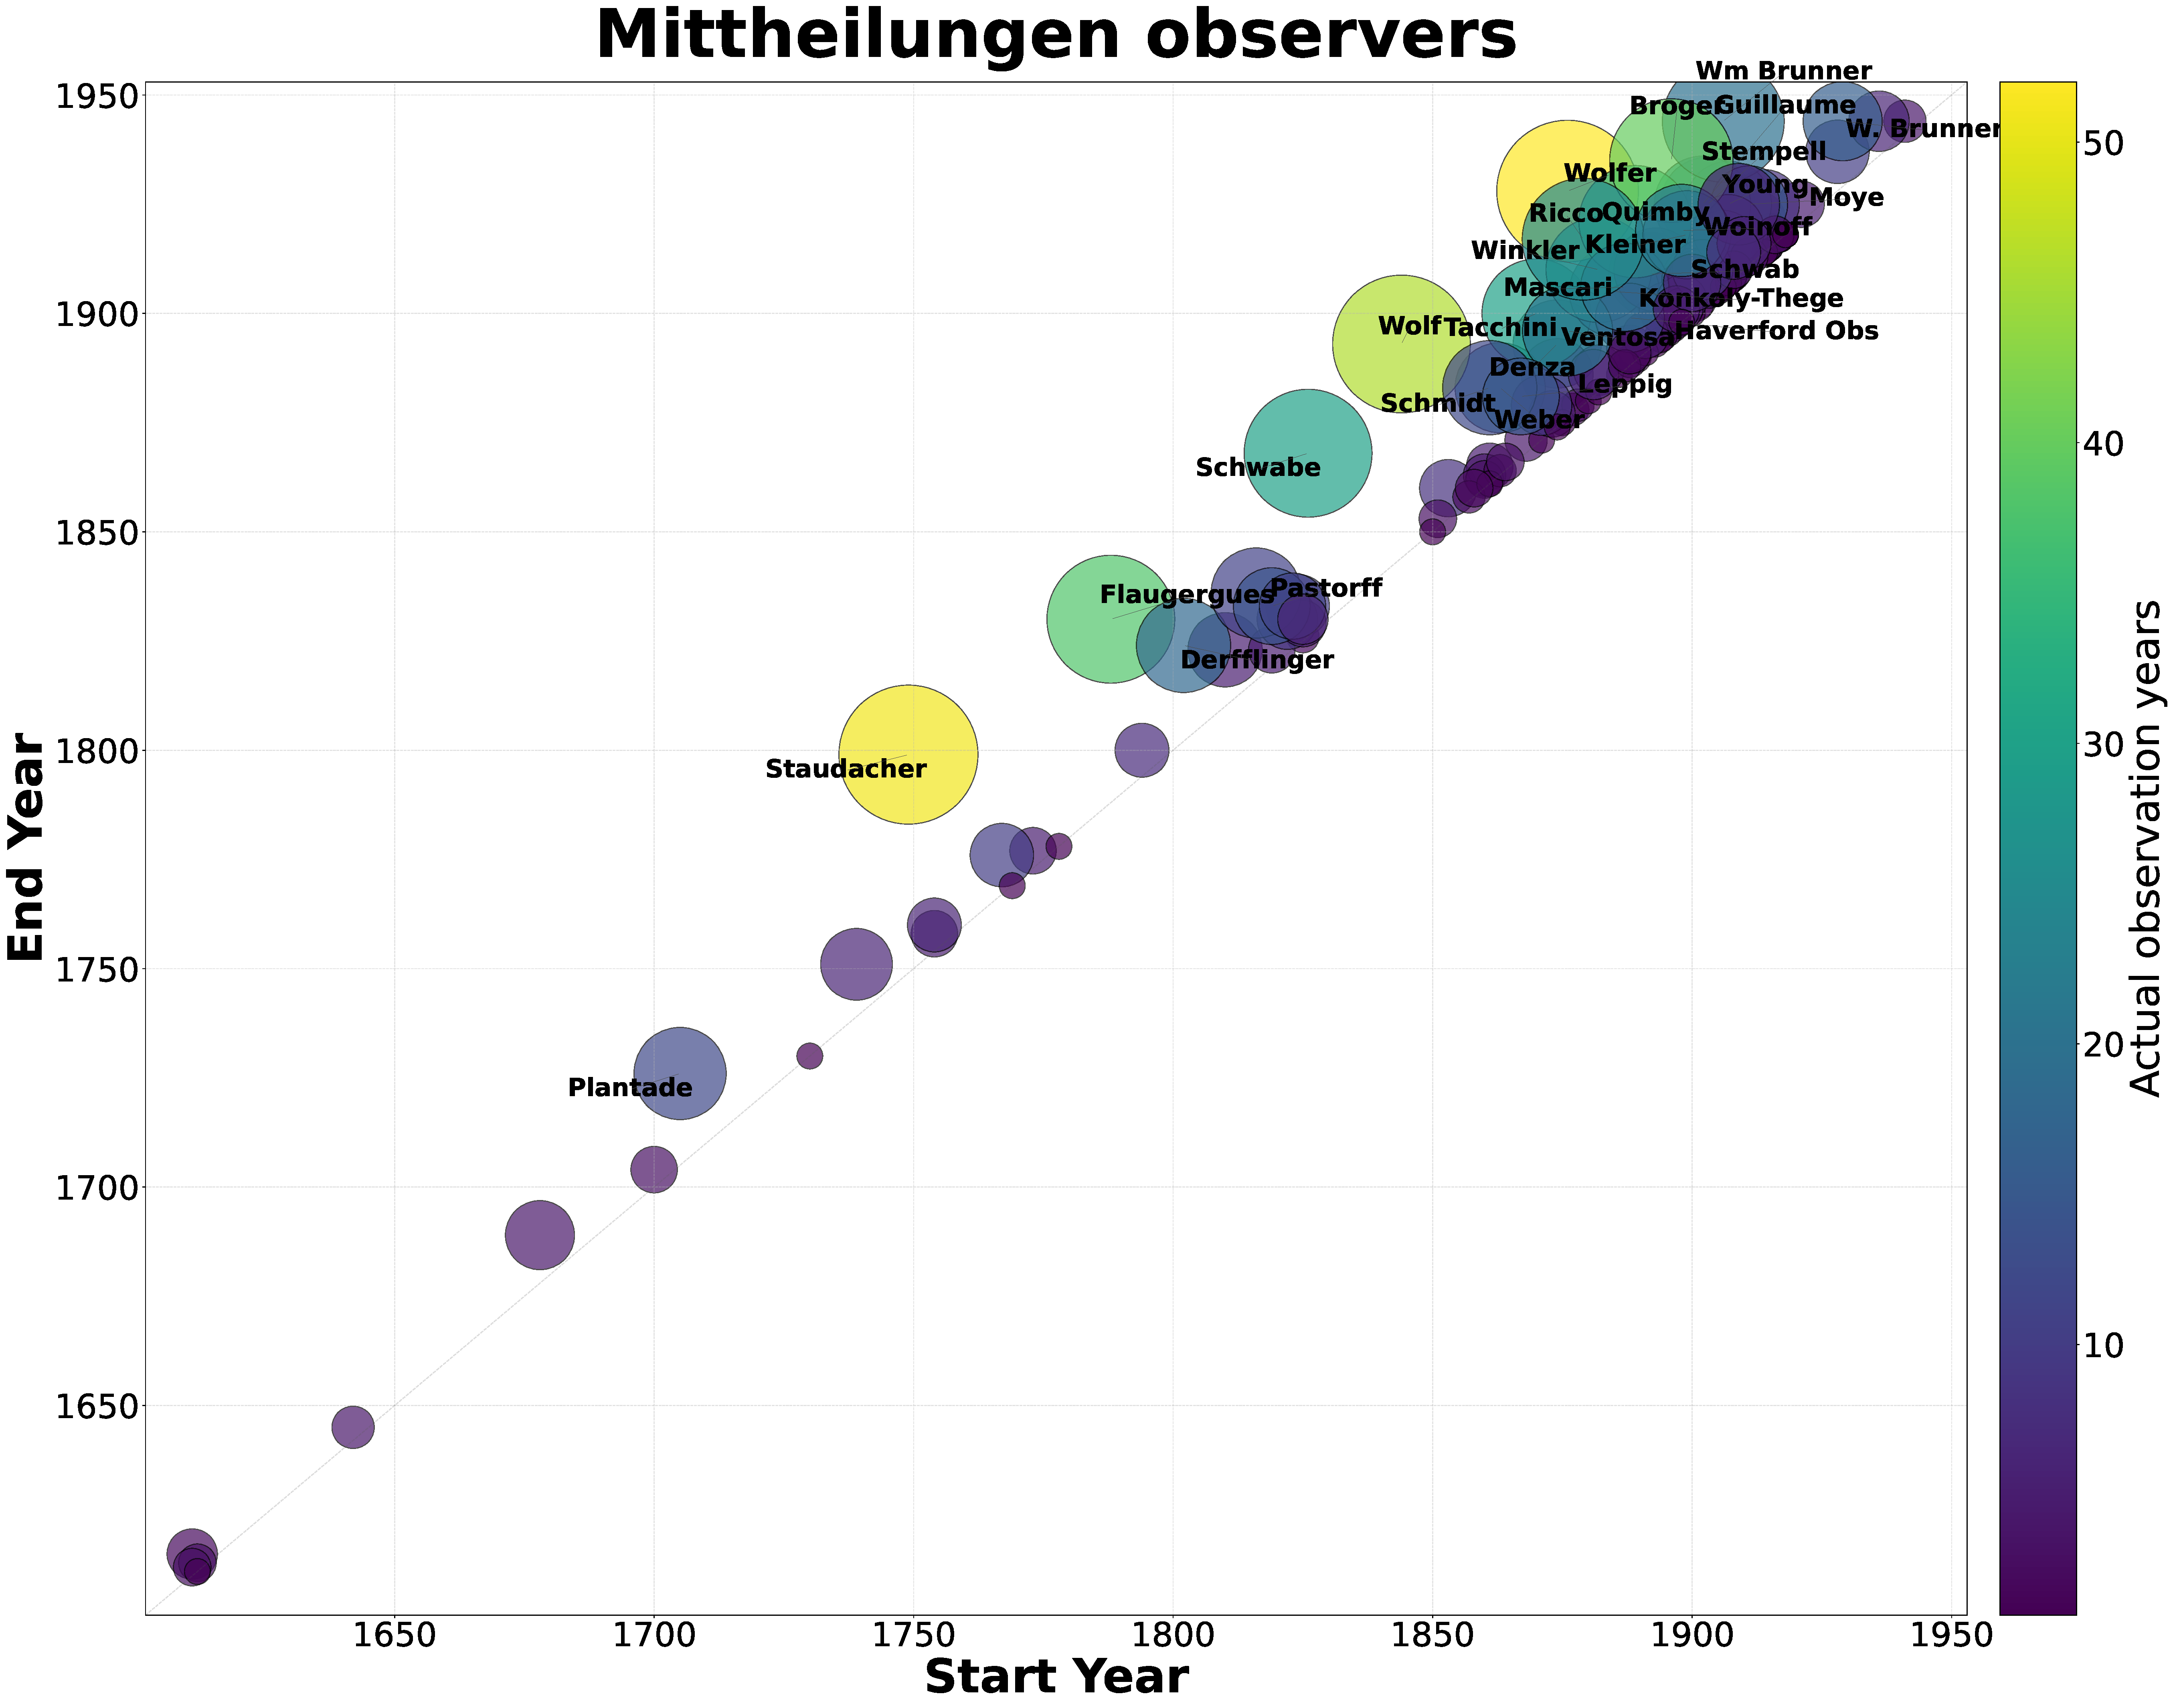
\includegraphics[width=\linewidth]{../figures/mitt_observer_bubble.pdf}
  \end{minipage}
\end{figure}

\vspace{-0.4em}

% ---------------------------------------------------------------
% ZURICH TABLES
% ---------------------------------------------------------------
\datasettab{Z\"urich Tables (1945--1979)}{\tabblue}

The Zürich Tables are the core record of SN production from 1945--1979.

\begin{itemize}
  \item 95\% digitised; detailed metadata 1945--1959 complete.
  \item Ongoing QC ensures consistent observer scaling.
\end{itemize}

% ---------------------------------------------------------------
% GRUITHUISEN
% ---------------------------------------------------------------
\datasettab{Gruithuisen Data (1817--1849)}{\taborange}

Gruithuisen manuscripts contain daily notes, drawings, and weather context in Kurrent script---critical for early-19th-century reconstruction.

\begin{itemize}
  \item Image + text sets fully collected.
  \item NG/NS verification underway.
\end{itemize}

\begin{figure}[t]
  \centering
  \begin{minipage}[t]{0.50\linewidth}
    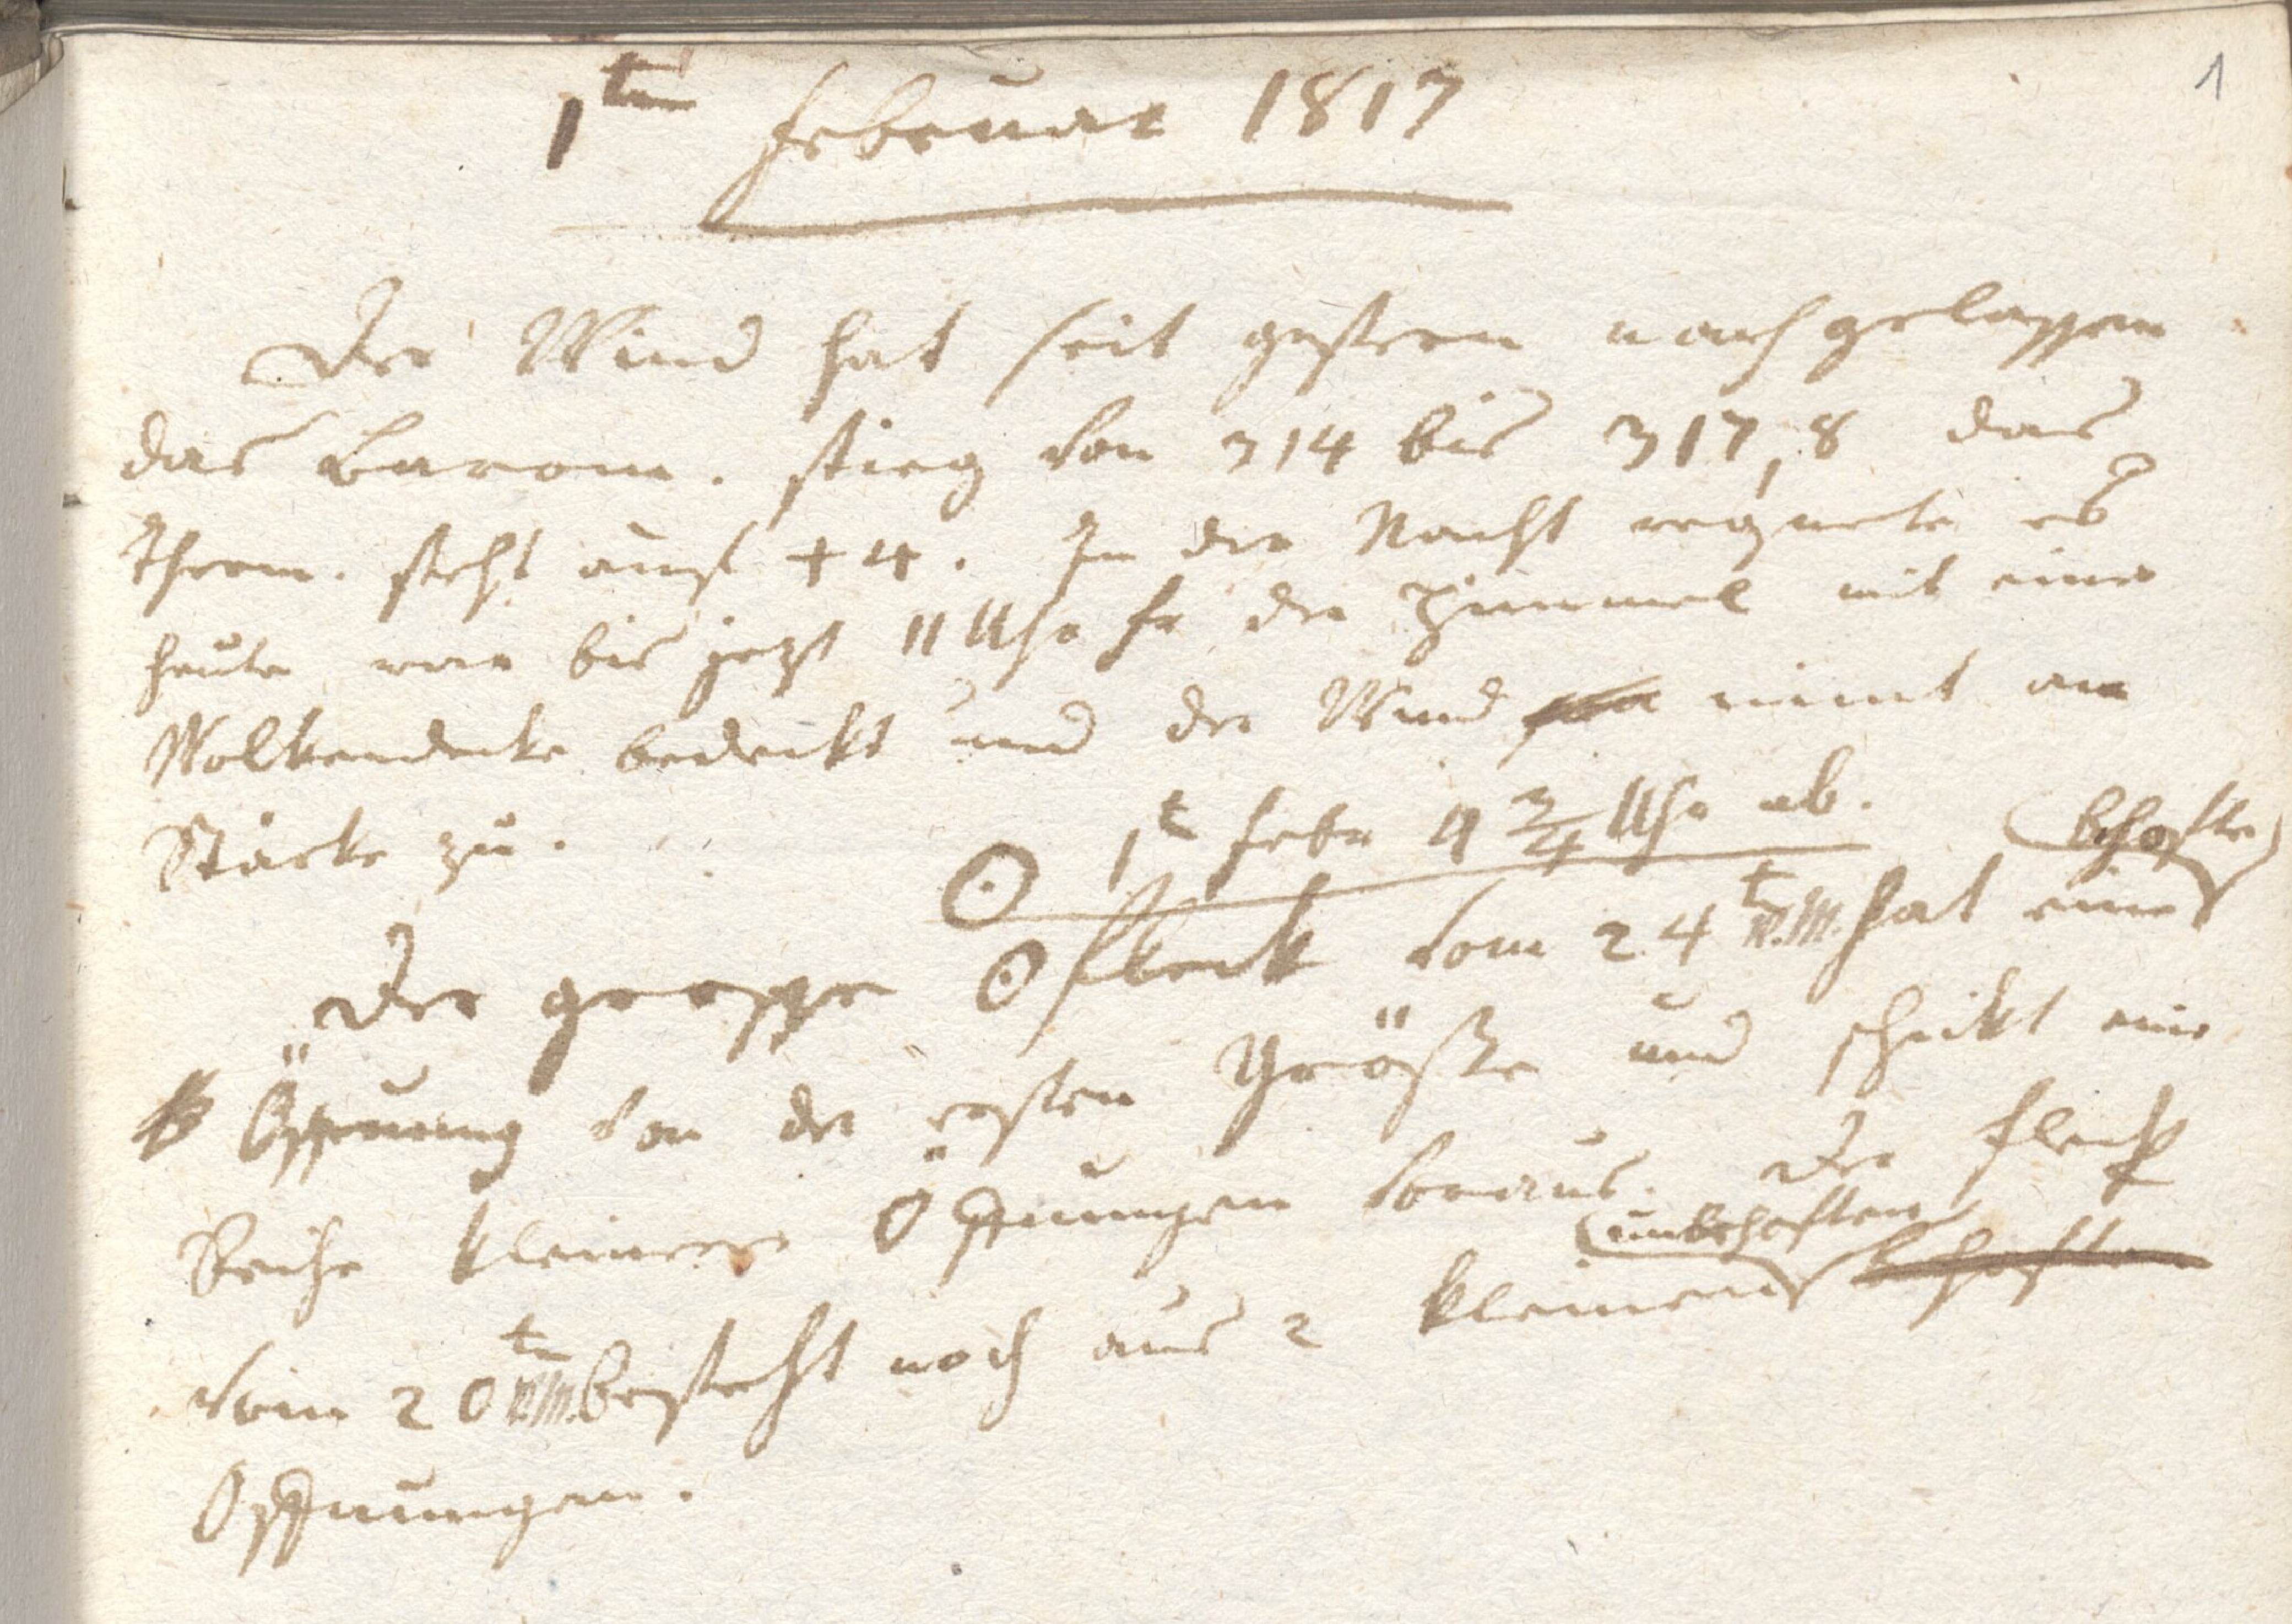
\includegraphics[width=\linewidth]{../figures/Gruithuisen_Sample1.png}
  \end{minipage}
  \hfill
  \begin{minipage}[t]{0.47\linewidth}
    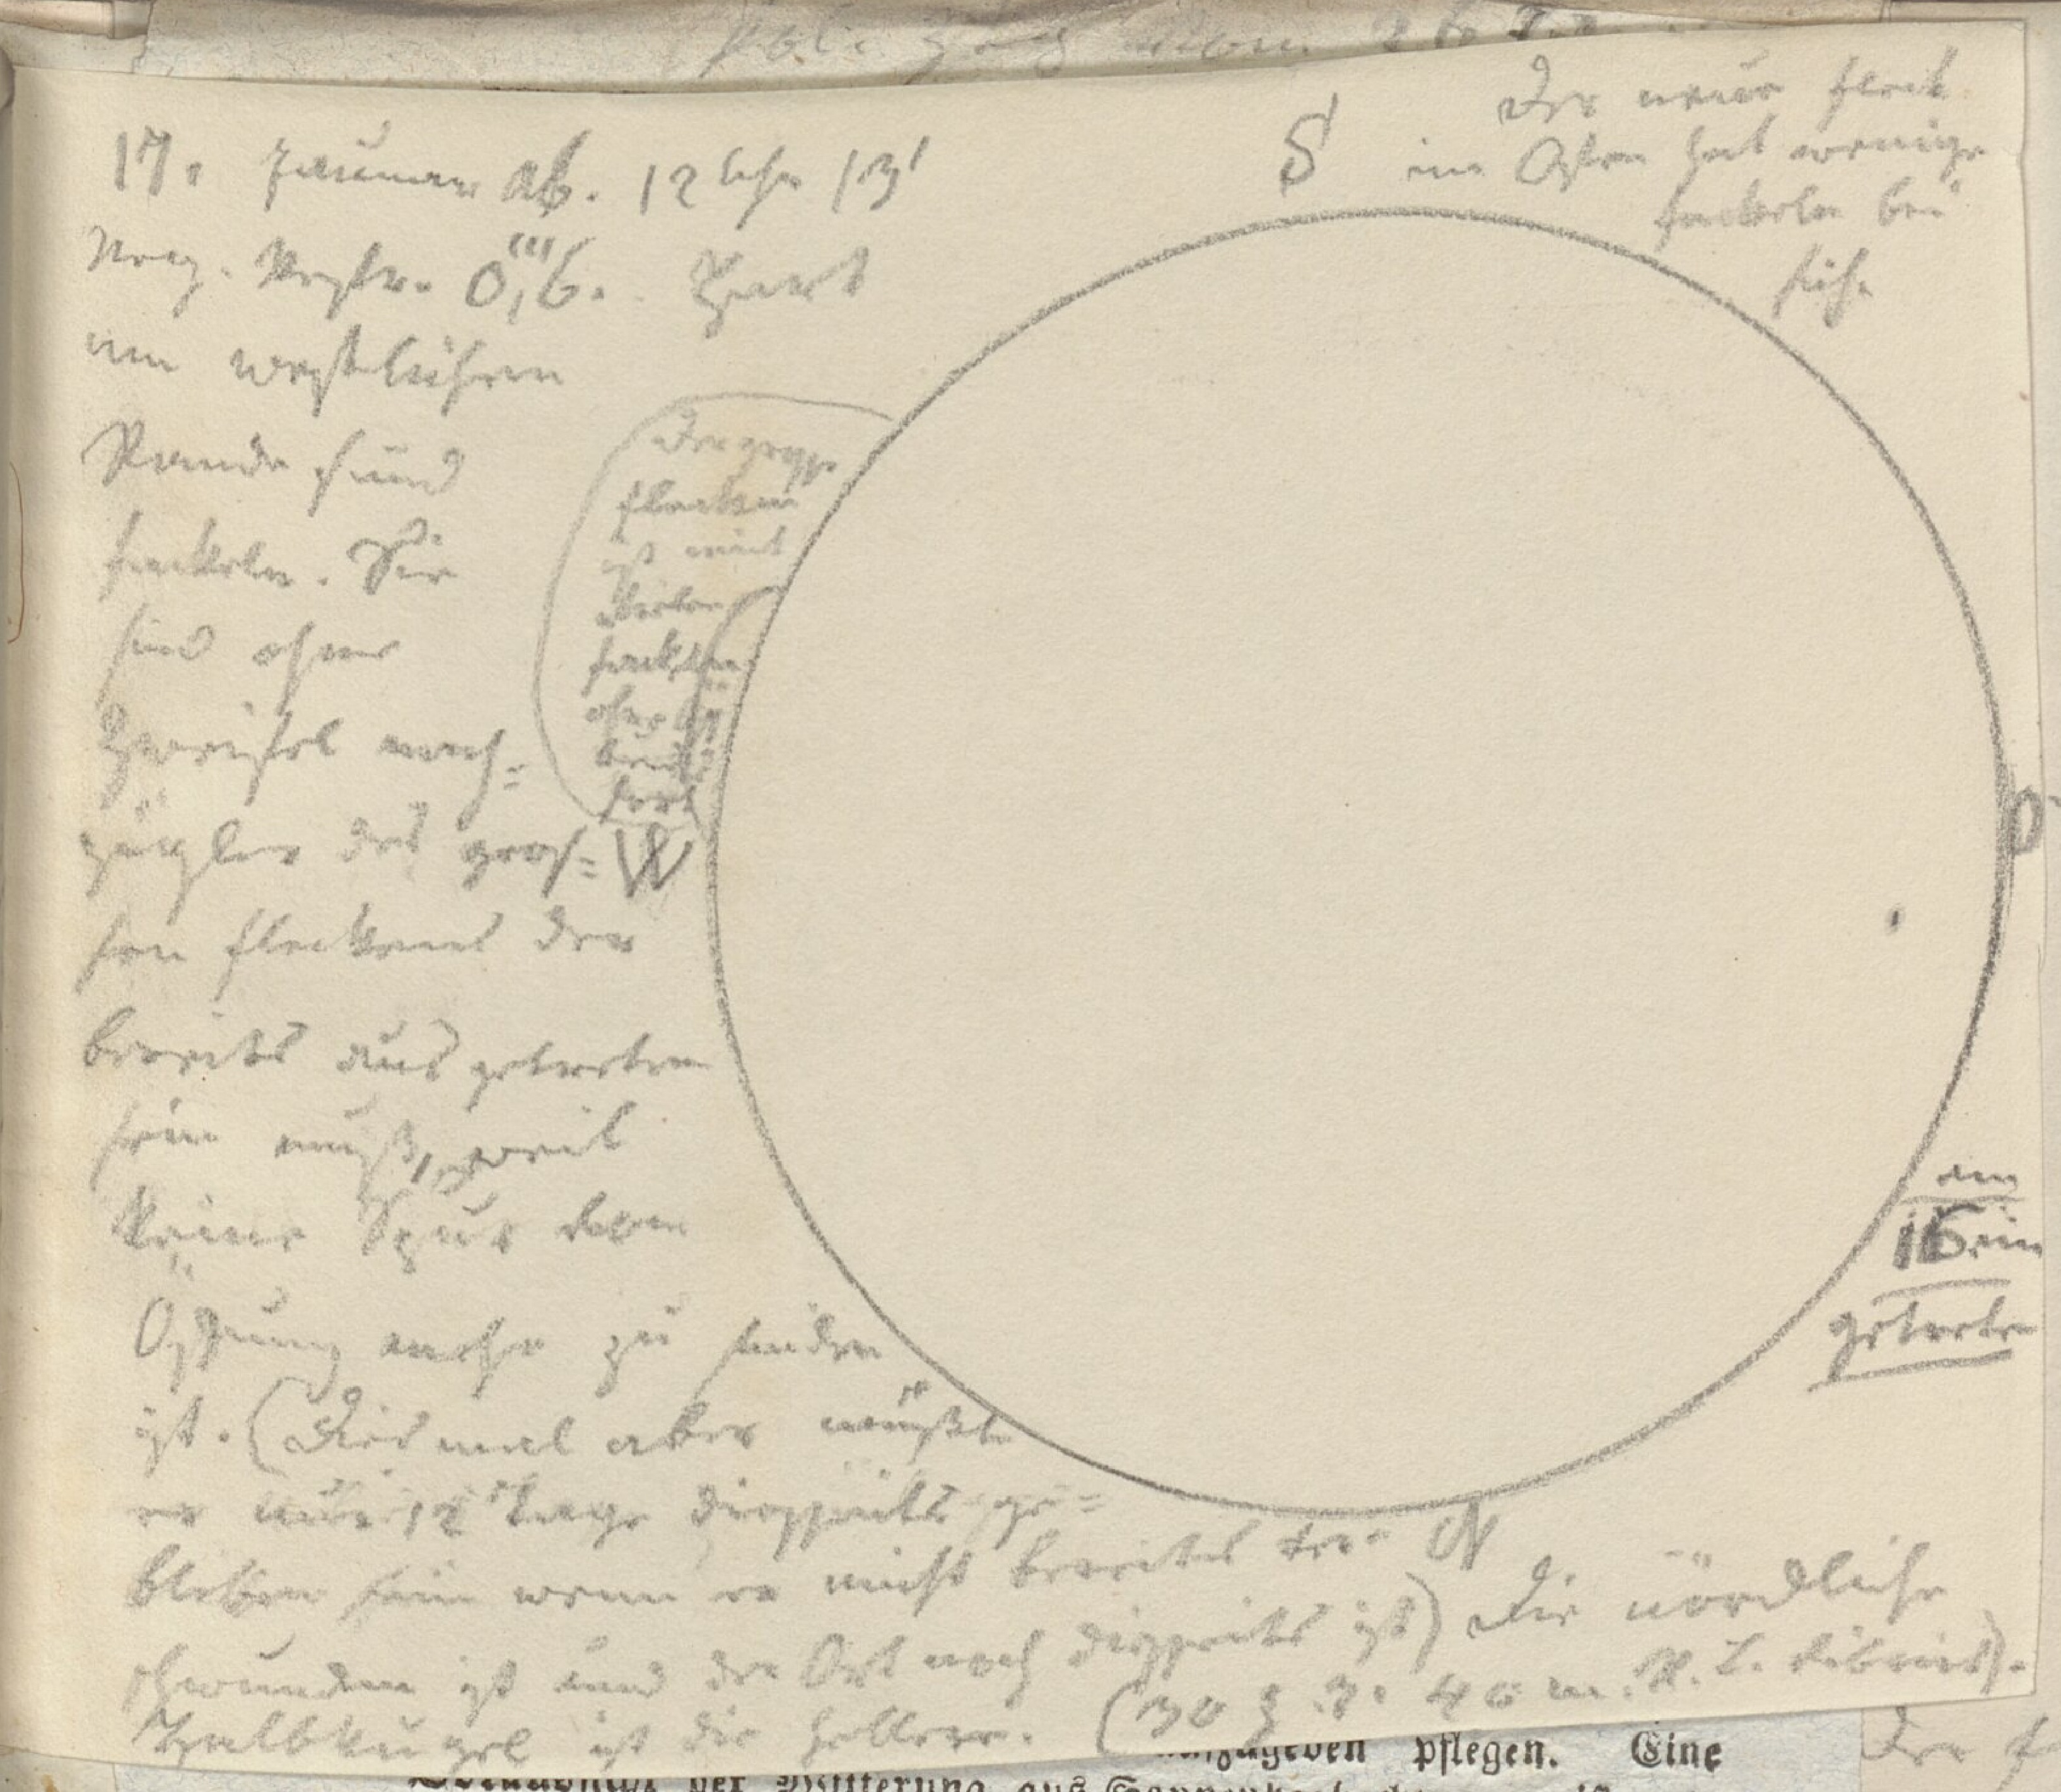
\includegraphics[width=\linewidth]{../figures/Gruithuisen_Sample2.jpg}
  \end{minipage}
\end{figure}

% ---------------------------------------------------------------
% ADAMS
% ---------------------------------------------------------------
\datasettab{C.~H.~Adams Data (1819--1823)}{\tabpurple}

Adams provides 338 drawings + 1,056 daily entries, including 748 spotless days useful for early-19th-century calibration.

\begin{itemize}
  \item Aligning direct vs reflection methods for calibration consistency.
  \item Preparing drawings for positional/area extraction.
\end{itemize}

\end{cardblock}

\end{column}


% *********************************************************************
% *********************************************************************
% COLUMN 3 --- RIGHT COLUMN
% *********************************************************************
% *********************************************************************

\begin{column}{0.26\paperwidth}
{\small

% ---------------------------------------------------------------
% STARK DATA
% ---------------------------------------------------------------
\begin{cardblock}{Key Datasets}

\datasettab{Augustin Stark Data (1813--1835)}{\tabred}

Stark's printed German descriptions of sunspot groups and chains provide valuable early-19th-century context. OCR trials show good potential; QC and metadata integration are ongoing.

% ---------------------------------------------------------------
% TIMELINE
% ---------------------------------------------------------------
\datasettab{Data Recovery Efforts Since 2010}{\tabgreen}

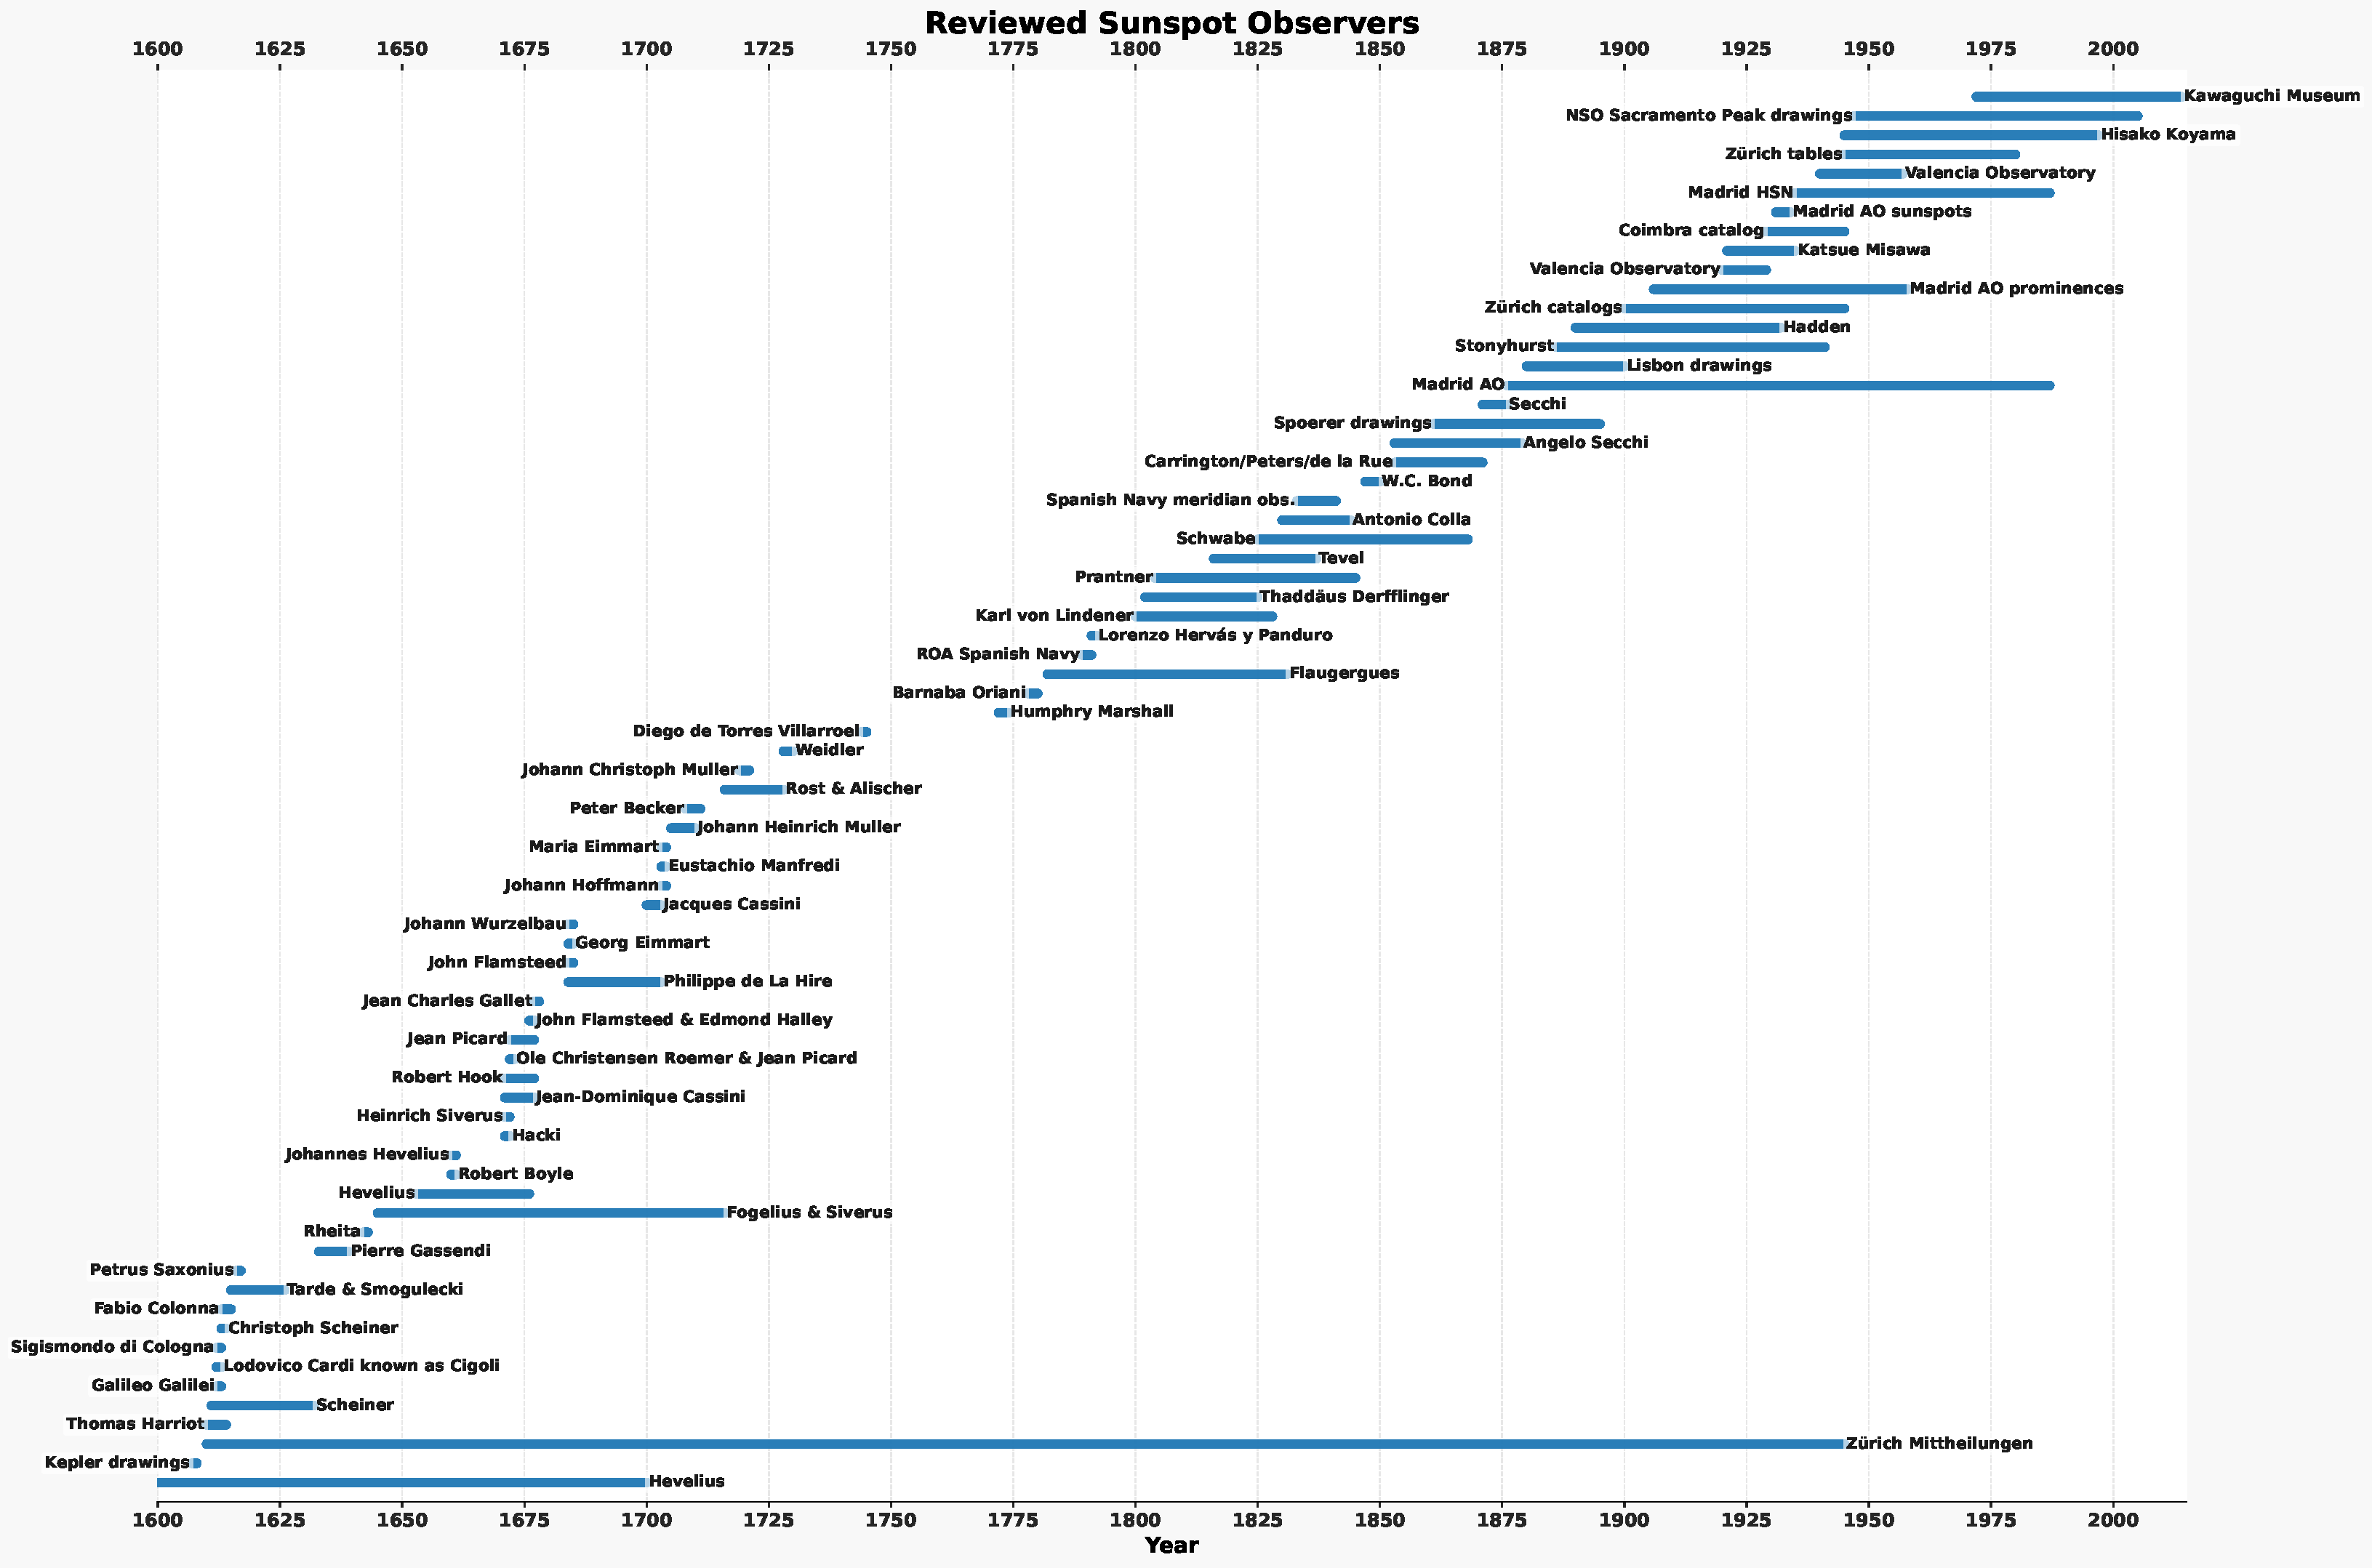
\includegraphics[width=\linewidth]{../figures/reviewed_sources_timeline_merged.pdf}

Community efforts since 2010 (Hayakawa, Arlt, Vaquero, Carrasco, etc.) have recovered many early telescopic datasets with broad temporal coverage.

\end{cardblock}

% ---------------------------------------------------------------
% PROGRESS HIGHLIGHTS
% ---------------------------------------------------------------
\begin{cardblock}{Progress Highlights}
\begin{itemize}
  \item Citizen-science portal blueprint prepared.
  \item Zürich pipeline blends HTR + manual review.
  \item Gruithuisen workflow combines experts + validation scripts.
  \item Adams spotless-day checks aligned with Mittheilungen.
\end{itemize}
\end{cardblock}

% ---------------------------------------------------------------
% RAW $\rightarrow$ V3.0 TRANSFORMATION
% ---------------------------------------------------------------
\begin{cardblock}{From Raw to SN V3.0}
\begin{enumerate}
  \item Curate observer metadata (instrument, weather, provenance).
  \item Solve observer response functions for group/spot alignment.
  \item Aggregate indices with uncertainty propagation.
  \item Benchmark against SN V2.0 and satellite-era proxies.
\end{enumerate}
\end{cardblock}

% ---------------------------------------------------------------
% CHALLENGES
% ---------------------------------------------------------------
\begin{cardblock}{Challenges}
\begin{itemize}
  \item Deciphering Kurrent handwriting while preserving context.
  \item Harmonising heterogeneous formats across centuries.
  \item Quantifying observer bias + spotless-day habits.
  \item Maintaining full provenance from scan $\rightarrow$ dataset $\rightarrow$ release.
\end{itemize}
\end{cardblock}

% ---------------------------------------------------------------
% SPACE CLIMATE IMPACT
% ---------------------------------------------------------------
\begin{cardblock}{Space Climate Impact}

\begin{minipage}[t]{0.48\linewidth}
  \callout{\color{AGUblue}Citizen Science}{
    Volunteers transcribe Kurrent manuscripts and contribute to STEM outreach.
  }
\end{minipage}
\hfill
\begin{minipage}[t]{0.48\linewidth}
  \callout{\color{AGUblue}Forecasting}{
    SN V3.0 improves solar cycle prediction and operational baselines.
  }
\end{minipage}

\vspace{0.25em}

\begin{minipage}[t]{0.48\linewidth}
  \callout{\color{AGUblue}Climate Links}{
    Improved long-term forcing helps refine climate models.
  }
\end{minipage}
\hfill
\begin{minipage}[t]{0.48\linewidth}
  \callout{\color{AGUblue}Open Science}{
    FAIR releases + APIs accelerate community reuse.
  }
\end{minipage}

\end{cardblock}

% ---------------------------------------------------------------
% QR CODE
% ---------------------------------------------------------------
\begin{cardblock}{Poster QR Code}
\centering

\includegraphics[width=1.3\linewidth]{../docs/figures/qrcode_farsun-poster.png}
\par\vspace{0.2em}
\small Scan for FARSuN information, datasets, and a digital copy of this poster.
\end{cardblock}

\vspace{-0.5em}
\par}
\end{column}

\end{columns}
\end{frame}
\end{document}

%
% % =====================================================================
% % Modern AGU-Style Poster --- Preamble Part 1A
% % Colors, fonts, global theme, minimal-flat foundation
% % =====================================================================
%
% \documentclass[final]{beamer}
%
% % ---- Beamerposter (A0 landscape) ----
% \usepackage[size=a0,orientation=landscape,scale=1.01]{beamerposter}
%
% % ---- Basic packages ----
% \usepackage[utf8]{inputenc}
% \usepackage[T1]{fontenc}
% \usepackage{lmodern}
% \usepackage{graphicx}
% \usepackage{booktabs}
% \usepackage{multicol}
% \usepackage{wrapfig}
% \usepackage{natbib}
% \bibliographystyle{unsrtnat}
% \usepackage{hyperref}
% \usepackage{array}
% \usepackage{ragged2e}
% \usepackage{xcolor}
% \usepackage{tcolorbox}
% \tcbuselibrary{skins,breakable}
% \usepackage{tikz}
% \usetikzlibrary{calc,decorations.pathreplacing}
%
% % -------------------------------------------------------------
% % 1. NEW AGU COLOR PALETTE (Palette A)
% % -------------------------------------------------------------
% \definecolor{AGUblue}{HTML}{0A2342}       % Deep navy
% \definecolor{AGUaqua}{HTML}{2EC4B6}       % Bright aqua accent
% \definecolor{AGUgold}{HTML}{FFBF69}       % Warm highlight gold
% \definecolor{AGUgray}{HTML}{F6F7F9}       % Soft card background
% \definecolor{AGUlight}{HTML}{FAFBFD}      % Ultra-light page wash
% \definecolor{AGUtext}{HTML}{1A1D1F}       % Neutral dark text
%
% % -------------------------------------------------------------
% % 2. GLOBAL TEXT & BACKGROUND CONFIG
% % -------------------------------------------------------------
% \setbeamercolor{normal text}{fg=AGUtext,bg=AGUlight}
% \setbeamercolor{structure}{fg=AGUaqua}
%
% % Sans-serif professional appearance (AGU style)
% \usefonttheme{professionalfonts}
% \renewcommand{\familydefault}{\sfdefault}
%
% % Paragraph spacing
% \setlength{\parskip}{0.3em}
% \setlength{\parindent}{0pt}
%
% % Column spacing
% \setlength{\columnsep}{2.0cm}
%
% % Softer, minimal background gradient
% \setbeamertemplate{background}{
%   \begin{tikzpicture}[remember picture,overlay]
%     \path[fill=AGUlight] (current page.south west)
%          rectangle (current page.north east);
%     \shade[top color=white, bottom color=AGUlight!60]
%          (current page.north west) rectangle
%          ($(current page.south east)+(0,8cm)$);
%   \end{tikzpicture}
% }
%
% % -----------------------------------------------------------------
% % Clean, readable text & title formatting
% % -----------------------------------------------------------------
% \setbeamerfont{title}{series=\bfseries,size=\Huge}
% \setbeamerfont{section title}{series=\bfseries,size=\Large}
% \setbeamerfont{block title}{series=\bfseries,size=\large}
%
% % Utilities
% \newcommand{\key}[1]{\textbf{\color{AGUaqua}#1}}
% \newcommand{\highlight}[1]{\textbf{\color{AGUgold}#1}}
%
% % =====================================================================
% % Modern AGU-Style Poster --- Preamble Part 1B
% % Minimal flat card blocks + dataset tabs
% % =====================================================================
%
% % ---------------------------------------------------------------------
% % 3. MAIN CARD BLOCK (flat, minimal, AGU-style)
% % ---------------------------------------------------------------------
% \newenvironment{cardblock}[1]{
%   \begin{tcolorbox}[
%       enhanced,
%       breakable,
%       colback=AGUgray,
%       colframe=AGUblue!5,
%       boxrule=0.4pt,
%       arc=2mm,
%       left=8pt,
%       right=8pt,
%       top=10pt,
%       bottom=8pt,
%       title={#1},
%       fonttitle=\bfseries\large\color{AGUblue},
%       coltitle=AGUblue,
%       attach boxed title to top left={yshift=-6pt,xshift=0pt},
%       boxed title style={
%         colback=AGUblue!10,
%         colframe=AGUblue!10,
%         arc=1mm,
%         boxrule=0pt,
%         top=4pt,
%         bottom=4pt,
%         left=6pt,
%         right=6pt,
%       }
%     ]
% }{
%   \end{tcolorbox}
% }
%
% % ---------------------------------------------------------------------
% % 4. “DATASET TAB” FLAT LABEL (replaces \datasetbox)
% % ---------------------------------------------------------------------
% \newcommand{\datasettab}[2]{%
%   \begin{tcolorbox}[
%       enhanced,
%       colback=AGUblue!4,
%       colframe=#2,
%       arc=1mm,
%       boxrule=1pt,
%       width=\linewidth,
%       left=6pt,
%       right=6pt,
%       top=4pt,
%       bottom=4pt,
%       sharp corners,
%     ]
%     {\bfseries\color{AGUblue}#1}
%   \end{tcolorbox}
% }
%
% % Color themes for dataset tabs
% \newcommand{\tabblue}{AGUaqua}
% \newcommand{\tabgreen}{AGUgold}
% \newcommand{\taborange}{AGUgold}
% \newcommand{\tabred}{AGUaqua!60!black}
% \newcommand{\tabpurple}{AGUblue!70}
%
% % ---------------------------------------------------------------------
% % 5. CALLOUT CARDS (flat, minimal)
% % ---------------------------------------------------------------------
% \newcommand{\callout}[2]{%
%   \begin{tcolorbox}[
%       colback=white,
%       colframe=AGUaqua,
%       arc=1.2mm,
%       boxrule=0.6pt,
%       left=6pt,
%       right=6pt,
%       top=4pt,
%       bottom=4pt,
%       width=\linewidth
%     ]
%     {\bfseries\color{AGUaqua}#1}\\[2pt]
%     {\small #2}
%   \end{tcolorbox}
% }
%
% % =====================================================================
% % Modern AGU-Style Poster --- Preamble Part 1C
% % Clean Header (Flat, Minimal)
% % =====================================================================
%
% \setbeamertemplate{headline}{
%   % -----------------------------------------------------------
%   % Flat navy bar background
%   % -----------------------------------------------------------
%   \begin{tikzpicture}[remember picture,overlay]
%     % Main navy header band
%     \path[fill=AGUblue]
%       (current page.north west)
%       rectangle ($(current page.north east)+(0,-7.5cm)$);
%
%     % Aqua underline stripe
%     \path[fill=AGUaqua]
%       ($(current page.north west)+(0,-7.5cm)$)
%       rectangle ($(current page.north east)+(0,-7.2cm)$);
%   \end{tikzpicture}
%
%   % -----------------------------------------------------------
%   % Title section with logos (kept same relative geometry)
%   % -----------------------------------------------------------
%   \begin{beamercolorbox}[wd=\paperwidth,ht=7.5cm,
%       leftskip=1.8cm,rightskip=1.8cm]{normal text}
%
%     \vspace{0.7cm}
%     \begin{minipage}[t]{0.17\paperwidth}
%       \vspace{0pt}
%       \centering
%       \includegraphics[height=4.2cm]{\leftlogo}
%     \end{minipage}
%     \hfill
%     \begin{minipage}[t]{0.53\paperwidth}
%       \vspace{0pt}
%       \raggedright
%       {\color{white}\bfseries\fontsize{46}{48}\selectfont \inserttitle}\\[0.55cm]
%       {\color{AGUgray!90!white}\Large \insertauthor}\\[0.25cm]
%       {\color{AGUgray!75!white}\normalsize \insertinstitute}
%     \end{minipage}
%     \hfill
%     \begin{minipage}[t]{0.23\paperwidth}
%       \vspace{0pt}
%       \raggedleft
%       \includegraphics[height=4.2cm]{\rightlogo}\hspace{0.4em}
%       \includegraphics[height=4.2cm]{\farsunlogo}
%     \end{minipage}
%   \end{beamercolorbox}
%
%   % -----------------------------------------------------------
%   % Session Badge (keep same placement but flat/minimal)
%   % -----------------------------------------------------------
%   \begin{tikzpicture}[remember picture,overlay]
%     \node[anchor=north west] at ($(current page.north west)+(0.4cm,-0.5cm)$) {
%       \begin{tcolorbox}[
%           enhanced,
%           colback=AGUgold!20,
%           colframe=AGUgold!60!AGUblue,
%           arc=2mm,
%           boxrule=0.7pt,
%           left=4mm,right=4mm,top=3mm,bottom=3mm,
%           width=0.17\paperwidth
%         ]
%         {\bfseries\small SH23E-2613* --- 16 Dec 2025\\[2pt]
%         \small Session: The Future of the International Sunspot Number}
%       \end{tcolorbox}
%     };
%   \end{tikzpicture}
%
%   \vspace{0.3cm}
% }
%
% % =====================================================================
% % Modern AGU-Style Poster --- Preamble Part 1D
% % Clean footer (flat, minimal)
% % =====================================================================
%
% \setbeamertemplate{footline}{
%   % -----------------------------------------------------------
%   % Flat navy footer bar
%   % -----------------------------------------------------------
%   \begin{tikzpicture}[remember picture,overlay]
%     \path[fill=AGUblue]
%       (current page.south west)
%       rectangle ($(current page.south east)+(0,1.9cm)$);
%
%     % Aqua accent stripe on top of the footer
%     \path[fill=AGUaqua]
%       ($(current page.south west)+(0,1.9cm)$)
%       rectangle ($(current page.south east)+(0,2.15cm)$);
%   \end{tikzpicture}
%
%   % -----------------------------------------------------------
%   % Footer text box (same geometry, modern typography)
%   % -----------------------------------------------------------
%   \begin{beamercolorbox}[wd=\paperwidth,ht=1.9cm,
%       leftskip=2.2cm,rightskip=2.2cm]{normal text}
%     \vspace{0.45cm}
%     {\Large
%       {\color{AGUaqua!95!white}\textbf{Contact:}} 
%       \href{mailto:sidc-support@oma.be}{\color{white}\textbf{sidc-support@oma.be}}
%       \hfill
%       {\color{AGUaqua!95!white}\textbf{Data Portal:}} 
%       \href{https://www.sidc.be/silso/}{\color{white}{https://www.sidc.be/silso/}}
%     }
%     \vspace{0.2cm}
%   \end{beamercolorbox}
% }
%
% % ================================================================
% % MESSAGE 2A --- COLUMN 1
% % ================================================================
%
% \begin{document}
% \begin{column}{0.28\paperwidth}
%
% % ------------------ ABSTRACT ------------------
% \begin{cardblock}{Abstract}
% \justifying
% The Sunspot Number (SN) is one of the longest continuous records of solar activity. SN V2.0 significantly improved the historical series through targeted recalibrations, but recent studies have shown that some scale changes---such as the 1849 transition---can only be fully understood by returning to the original raw observations. This motivates a complete reconstruction (SN V3.0) in which uncertainties and calibration steps arise directly from the quality of each dataset rather than from global statistical corrections.
%
% To enable this reconstruction, the historical data foundation has expanded dramatically in recent years. WDC--SILSO digitized the Mittheilungen (1610--1944) between 2017 and 2019, converting Wolf's original Zürich journals into machine-readable datasets with modern metadata and provenance. As part of FARSuN, the Zürich observation tables for 1945--1979 were digitized from 2023 to 2025, completing the recovery of the full Zürich legacy. In parallel, major community efforts (e.g., Hayakawa, Arlt, Vaquero, Carrasco) have located, transcribed, and published numerous additional early telescopic sunspot records since 2010.
%
% Together, these datasets greatly expand the number of overlapping observations and allow independent cross-checks across observers and epochs. This richer observational base strengthens scale-transfer analyses, improves calibration robustness, and provides the foundation for an uncertainty-quantified reconstruction of the long-term sunspot series. These advances make a defensible SN V3.0 possible and ensure that the Sunspot Number remains a reliable reference for solar activity studies.
% \end{cardblock}
%
% % ------------------ FOUR-AXIS METHOD ------------------
% \begin{cardblock}{Four-Axis Methodology}
% \begin{enumerate}
%   \item \key{Gather Sources}: track down dispersed observing logs (Wolf's \emph{Mittheilungen}, Zürich tables, Gruithuisen manuscripts, Adams drawings) and capture provenance metadata at ingest.
%   \item \key{Process Data}: use handwriting/OCR engines (Transkribus models, custom scripts) alongside manual double-keying for fragile entries.
%   \item \key{Validate \& Standardize}: reconcile aliases, observer IDs, and calendars; model group/spot counting behaviour to derive calibration curves.
%   \item \key{Disseminate}: publish machine-readable products, APIs, and VO-ready services with versioned uncertainty bundles for each release.
% \end{enumerate}
% \end{cardblock}
%
% % ------------------ FARSUN DATABASE ------------------
% \begin{cardblock}{FARSuN Historical Sunspot Database}
% A sustainable, interoperable reference ensuring that four centuries of solar observations remain accessible and scientifically reliable for future Sun--climate research.
%
% \begin{itemize}
%   \item Legacy sources (Mittheilungen, Wolf Institute, Adams, Gruithuisen, Stark) integrated into the schema for cross-validation and QC.
%   \item Automated QC detects inconsistencies (NG > NS, duplicates, missing metadata).
%   \item Metadata harmonization underway for observers, instruments, and observatories.
% \end{itemize}
%
% \textbf{Next Steps}
% \begin{itemize}
%   \item Finalize canonical schema and close remaining legacy mappings.
%   \item Expand QC dashboards and uncertainty modeling.
%   \item Scale up digitization/extraction (Adams, Gruithuisen, Stark) using HTR and citizen-science workflows.
%   \item Expose dataset via EPN-TAP for FAIR access.
%   \item Use this harmonized database as the foundation for SN V3.0 calibration.
% \end{itemize}
% \end{cardblock}
%
% % ------------------ METHODS ------------------
% \begin{cardblock}{Methods}
% \begin{itemize}
%   \item Dual-mode transcription: Transkribus handwriting models + manual keying.
%   \item Data hygiene: reconcile aliases, calendars, recount audits.
%   \item Uncertainty modelling: propagate observer response functions.
%   \item Automation: reproducible Python pipelines with QC checkpoints.
% \end{itemize}
% \end{cardblock}
%
% % ------------------ QUALITY GATES ------------------
% \begin{cardblock}{Quality Gates}
% \begin{itemize}
%   \item Two-person verification for Adams and Gruithuisen entries.
%   \item Cross-compare with Mittheilungen and SILSO indices for drift detection.
%   \item Metadata harmonisation ensures unique observer IDs and instrument notes.
%   \item Git-tracked pipelines record all transformations for audit and reuse.
% \end{itemize}
% \end{cardblock}
%
% \end{column}
%
% % ================================================================
% % MESSAGE 2B --- COLUMN 2
% % ================================================================
%
% \begin{column}{0.42\paperwidth}
%
% \begin{cardblock}{Key Datasets}
%
% % ------------------ MITTHEILUNGEN ------------------
% \datasettab{Mittheilungen Dataset (1610--1945)}{\tabgreen}
%
% \begin{figure}[t]
%   \centering
%   \begin{minipage}[t]{0.45\linewidth}
%     \vspace{0pt}
%     The Mittheilungen journals, compiled by Rudolf Wolf and successors at the Zürich Observatory, form a central source of historical sunspot observations. They document daily group and spot counts from 1848 to 1945 and incorporate earlier material back to 1610 through Wolf's compilations.
%
%     Within FARSuN, the full series was digitized and structured at the Royal Observatory of Belgium and is being checked for metadata consistency and observer alignment.
%     \begin{itemize}
%       \item Refining data consistency and observer calibration (Wolf--Wolfer overlap).
%       \item Finalizing metadata alignment for FAIR publication.
%       \item Resolving remaining ID and provenance issues.
%     \end{itemize}
%   \end{minipage}
%   \hfill
%   \begin{minipage}[t]{0.52\linewidth}
%     \vspace{0pt}
%     \centering
%     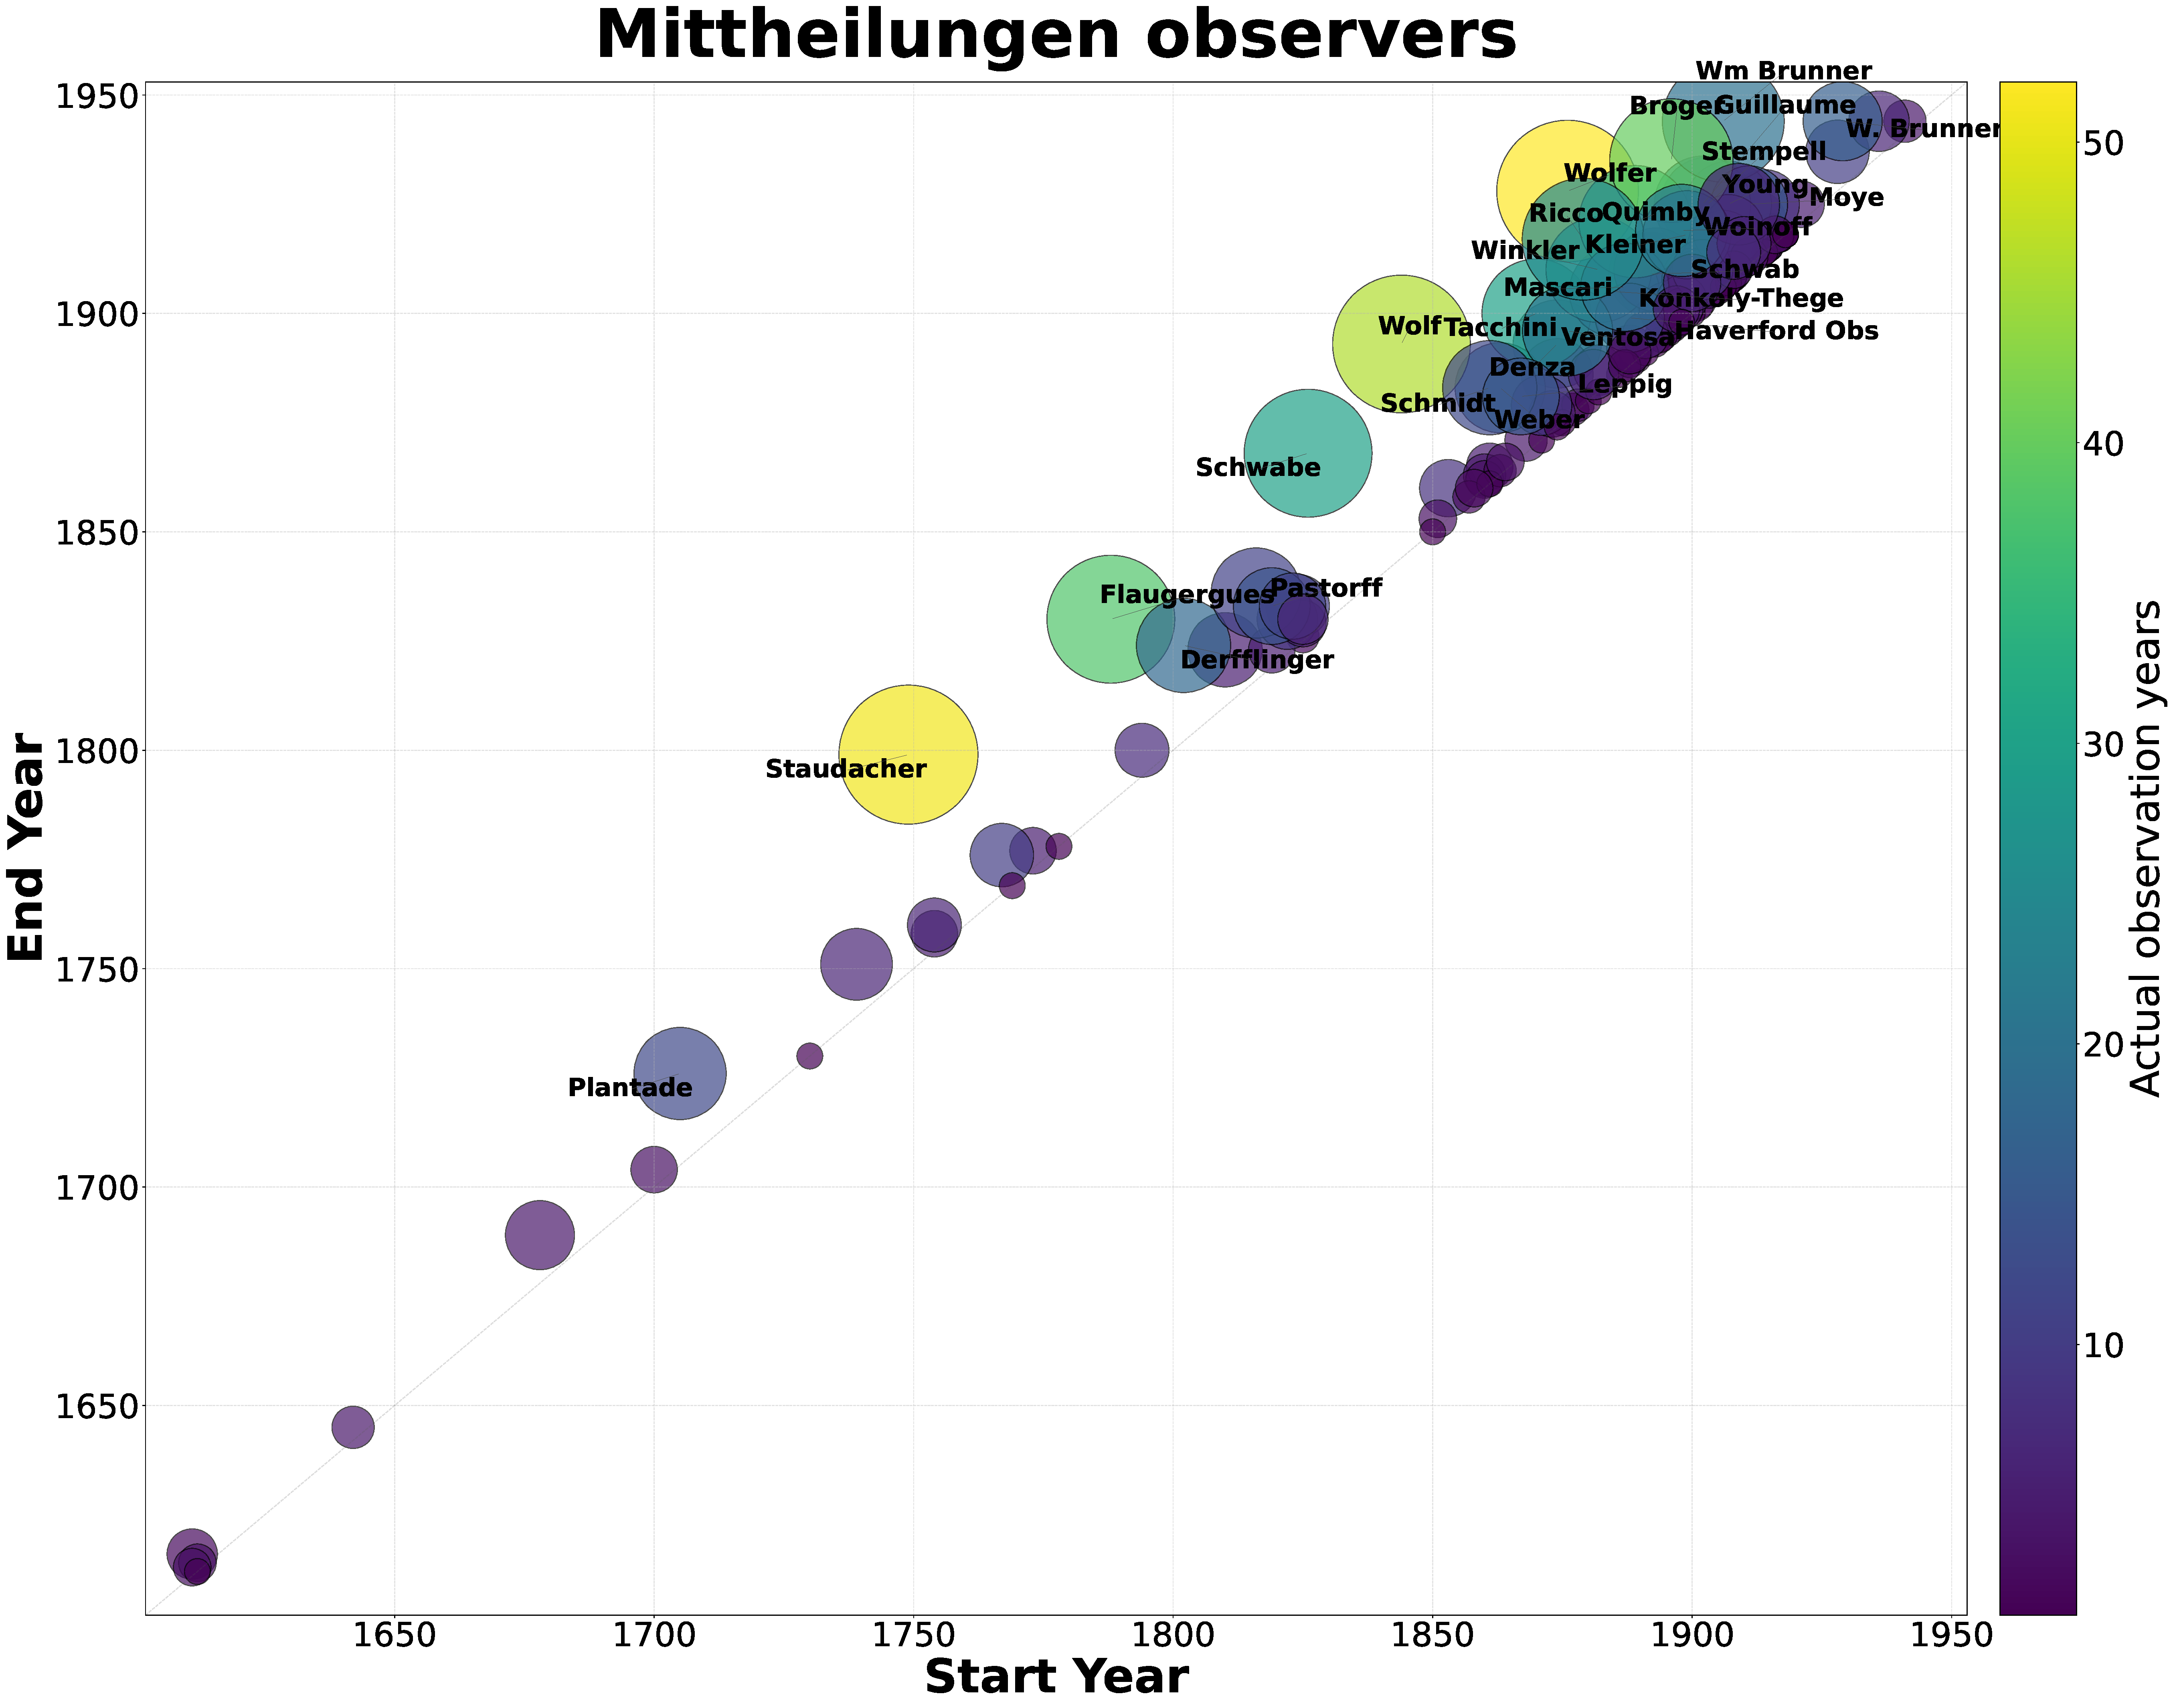
\includegraphics[width=\linewidth]{../figures/mitt_observer_bubble.pdf}
%   \end{minipage}
% \end{figure}
%
% \vspace{-0.6em}
%
% % ------------------ ZURICH TABLES ------------------
% \datasettab{Z\"urich Tables (1945--1979)}{\tabblue}
%
% \vspace{0.2cm}
% The Z\"urich Tables form the foundational record of daily sunspot number production at the Zürich Observatory between 1945 and 1979.
%
% \textit{Status}: 95\% of the 2\,000+ yearly tables are digitized and late-1970s metadata encoding is nearly complete.
%
% \begin{itemize}
%   \item Fully digitized for 1945--1979 with detailed metadata completed for 1945--1959.
%   \item Quality control and observer metadata harmonization underway.
% \end{itemize}
%
% % ------------------ GRUITHUISEN ------------------
% \datasettab{Gruithuisen Data (1817--1849)}{\taborange}
%
% \vspace{0.3em}
% The Gruithuisen manuscripts capture daily sunspot notes, drawings, and weather context in German Kurrent script---critical for early-19th-century SN calibration.
%
% \begin{itemize}
%   \item Image sets and text snippets fully collected with preliminary CSV/XLSX extraction completed.
%   \item Two-pass QC (survey + counting) underway for verified NG/NS tallies.
% \end{itemize}
%
% \begin{figure}[t]
%   \centering
%   \begin{minipage}[t]{0.50\linewidth}
%     \centering
%     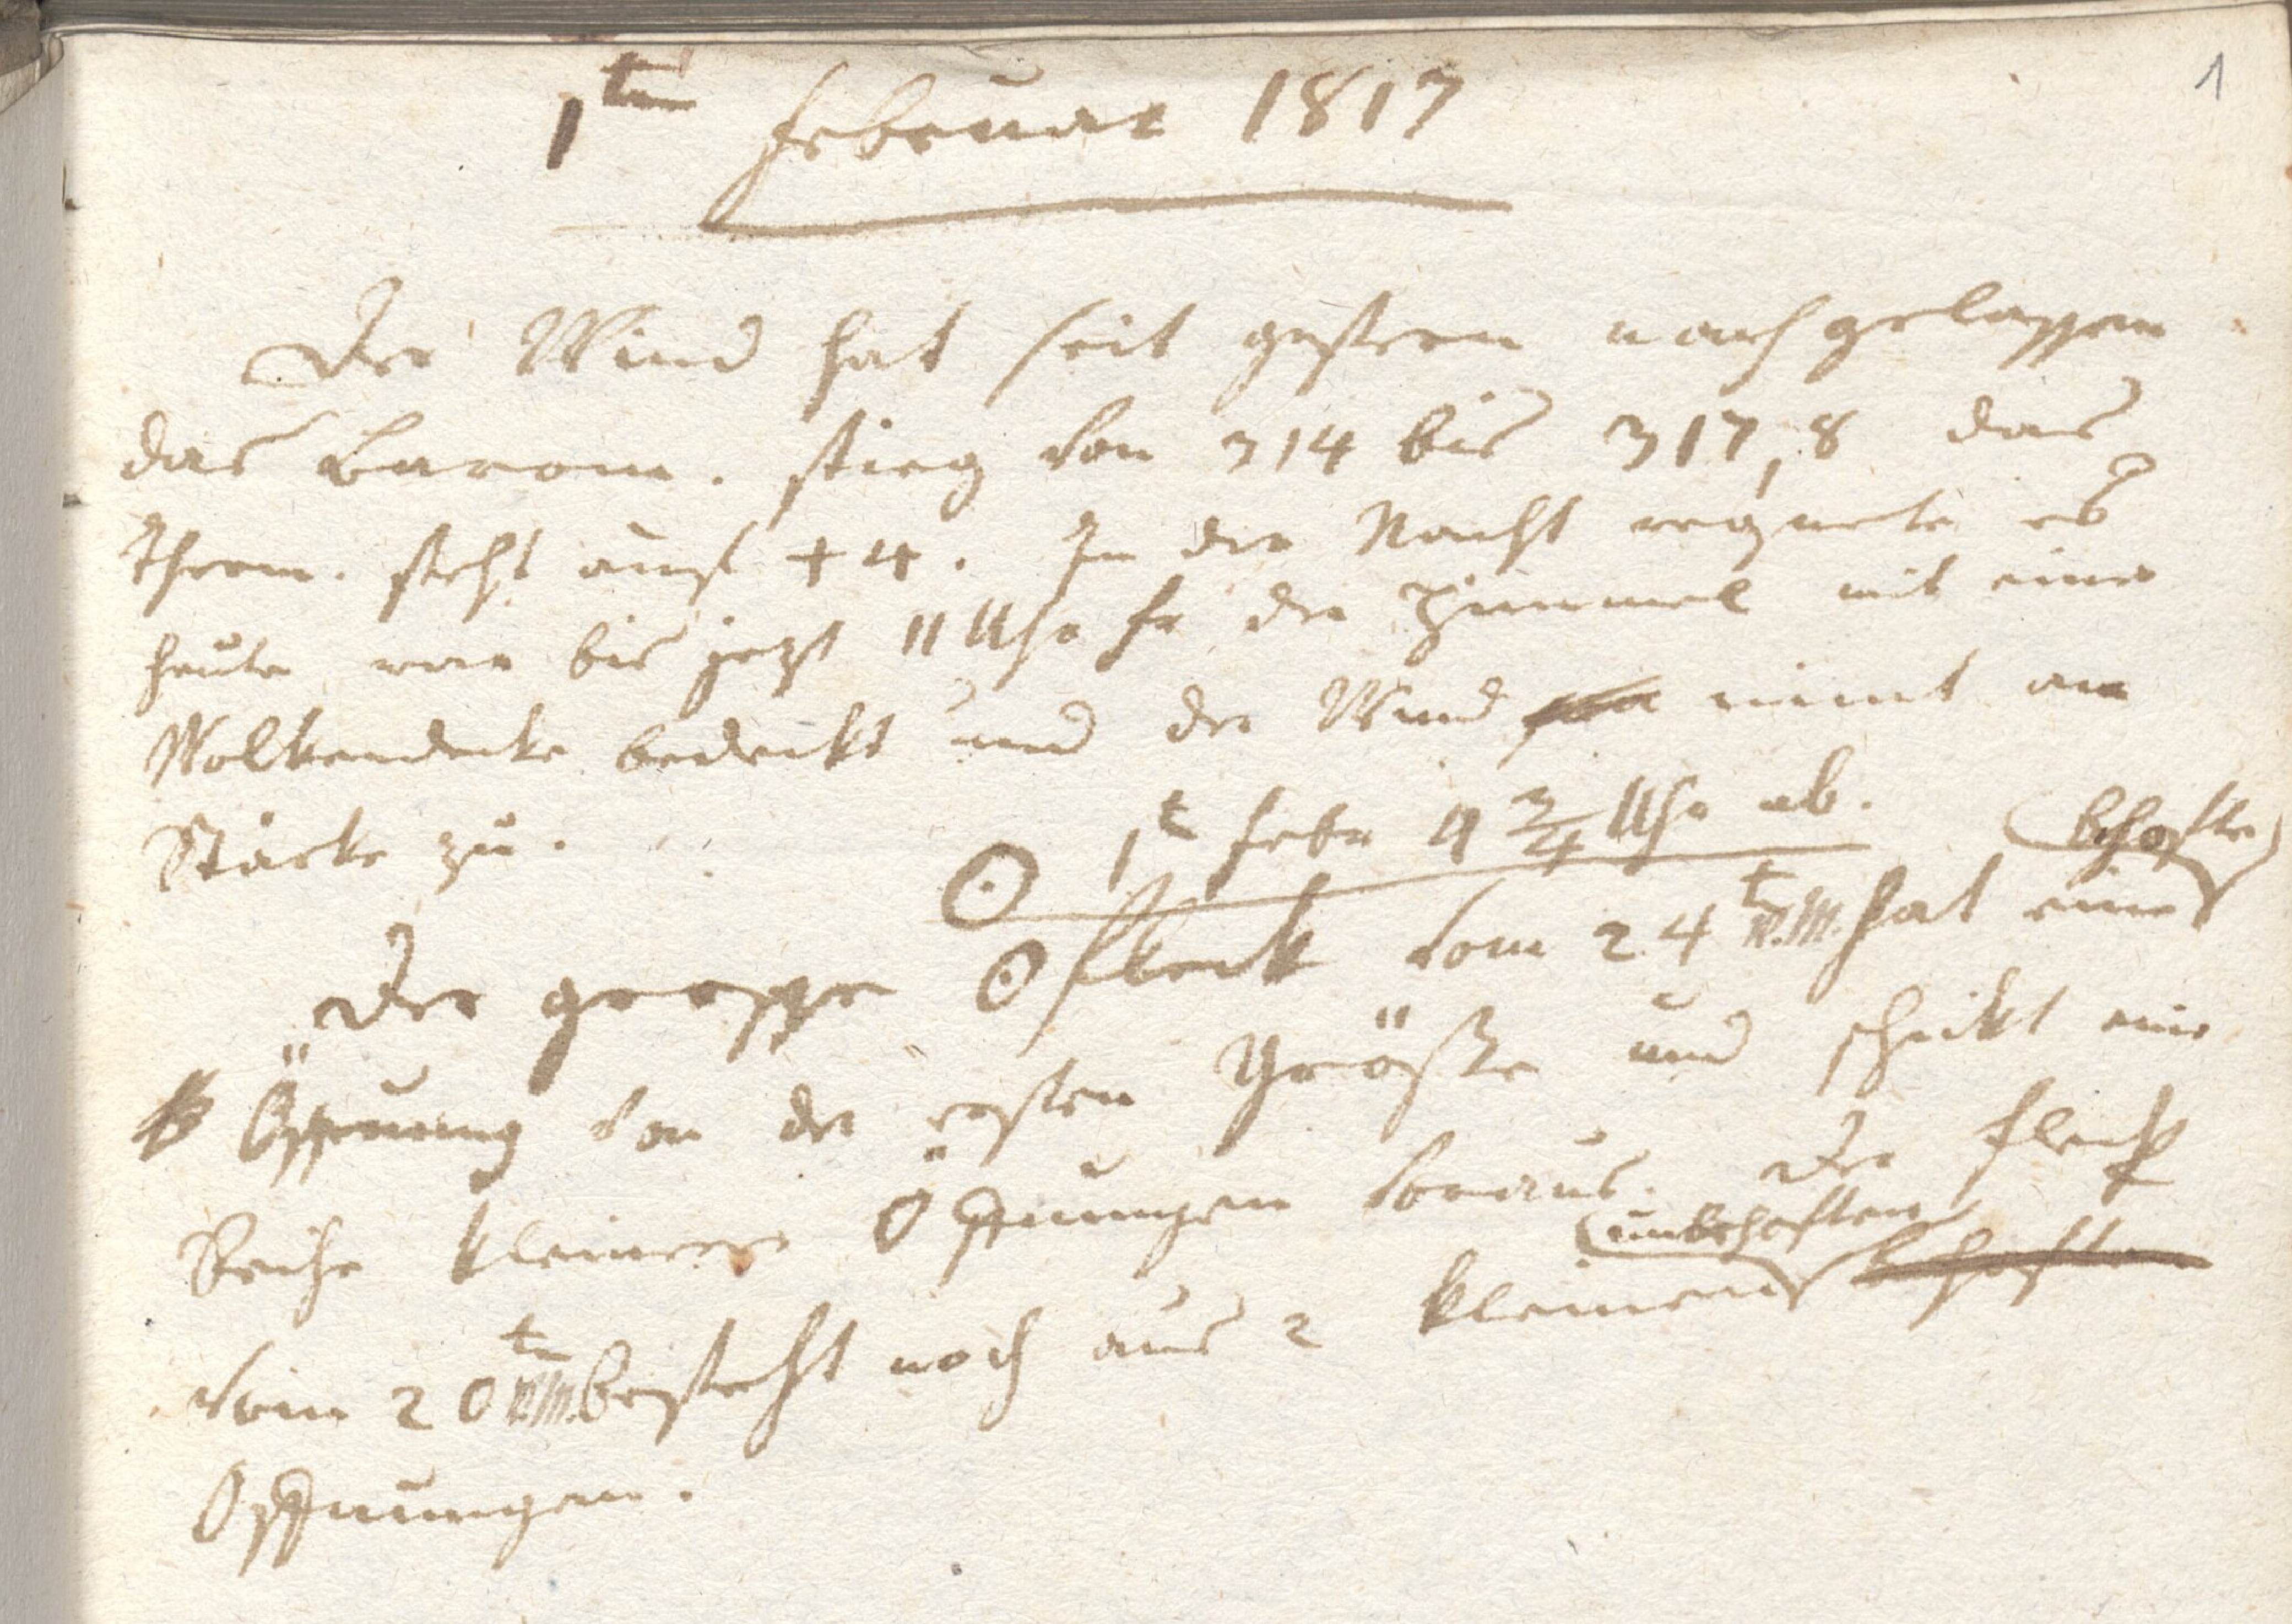
\includegraphics[width=\linewidth]{../figures/Gruithuisen_Sample1.png}
%   \end{minipage}
%   \hfill
%   \begin{minipage}[t]{0.47\linewidth}
%     \centering
%     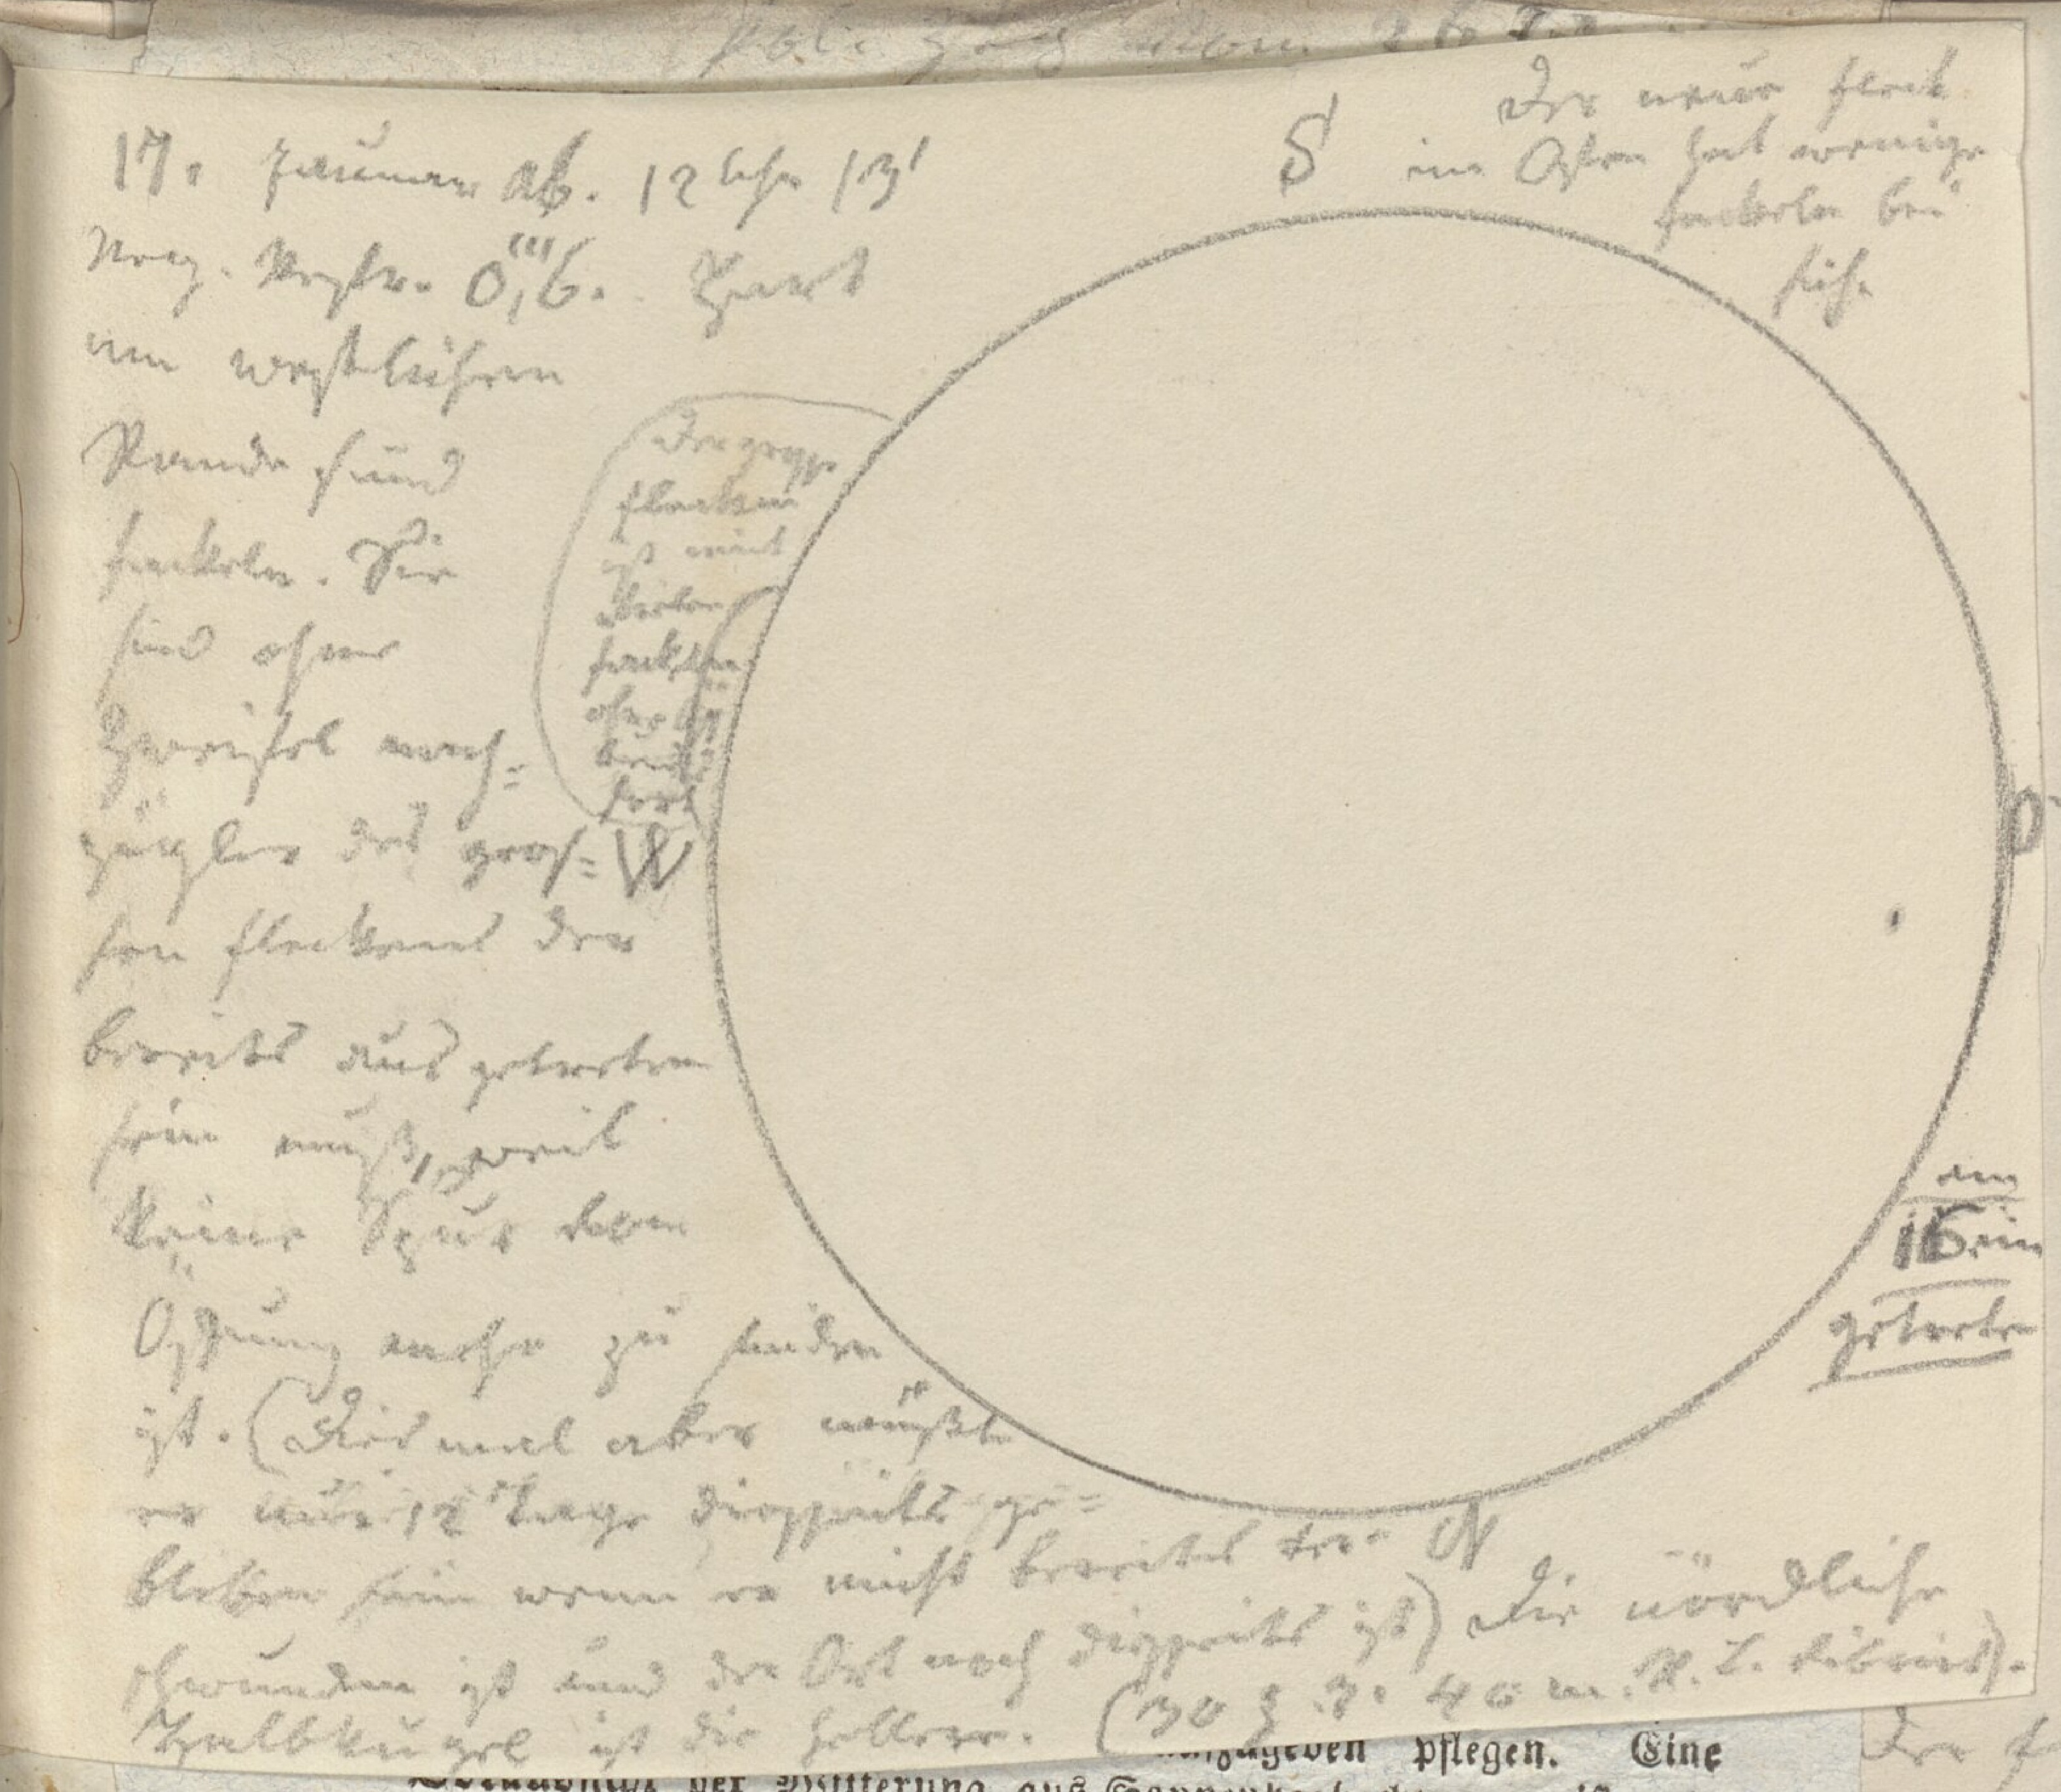
\includegraphics[width=\linewidth]{../figures/Gruithuisen_Sample2.jpg}
%   \end{minipage}
% \end{figure}
%
% % ------------------ ADAMS ------------------
% \datasettab{C.~H.~Adams Data (1819--1823)}{\tabpurple}
%
% FARSuN has recovered 338 full-disk drawings and 1,056 daily entries (308 spot days, 748 spotless) from C.~H. Adams, providing dense coverage with explicit spotless days.
%
% \begin{itemize}
%   \item Quality checks to align direct and reflection methods for consistent calibration.
%   \item Standardisation of drawings to enable positional and area extractions later.
% \end{itemize}
%
% \end{cardblock}
%
% \end{column}
%
% % ================================================================
% % MESSAGE 2C --- COLUMN 3
% % ================================================================
%
% \begin{column}{0.26\paperwidth}
% {\small
%
% % ------------------ STARK DATA ------------------
% \begin{cardblock}{Key Datasets}
%
% \datasettab{Augustin Stark Data (1813--1835)}{\tabred}
%
% The Stark dataset (1813--1835), comprising printed German descriptions of sunspot groups and chains, has been partially retrieved. Preliminary OCR tests show good potential, and ongoing work focuses on QC flags and metadata integration into the FARSuN database. Extraction campaigns continue to ensure descriptive passages are tagged consistently before ingestion.
%
% % ------------------ TIMELINE OF DATA RECOVERY ------------------
% \datasettab{Data Recovery Efforts Since 2010}{tabgreen}
%
% 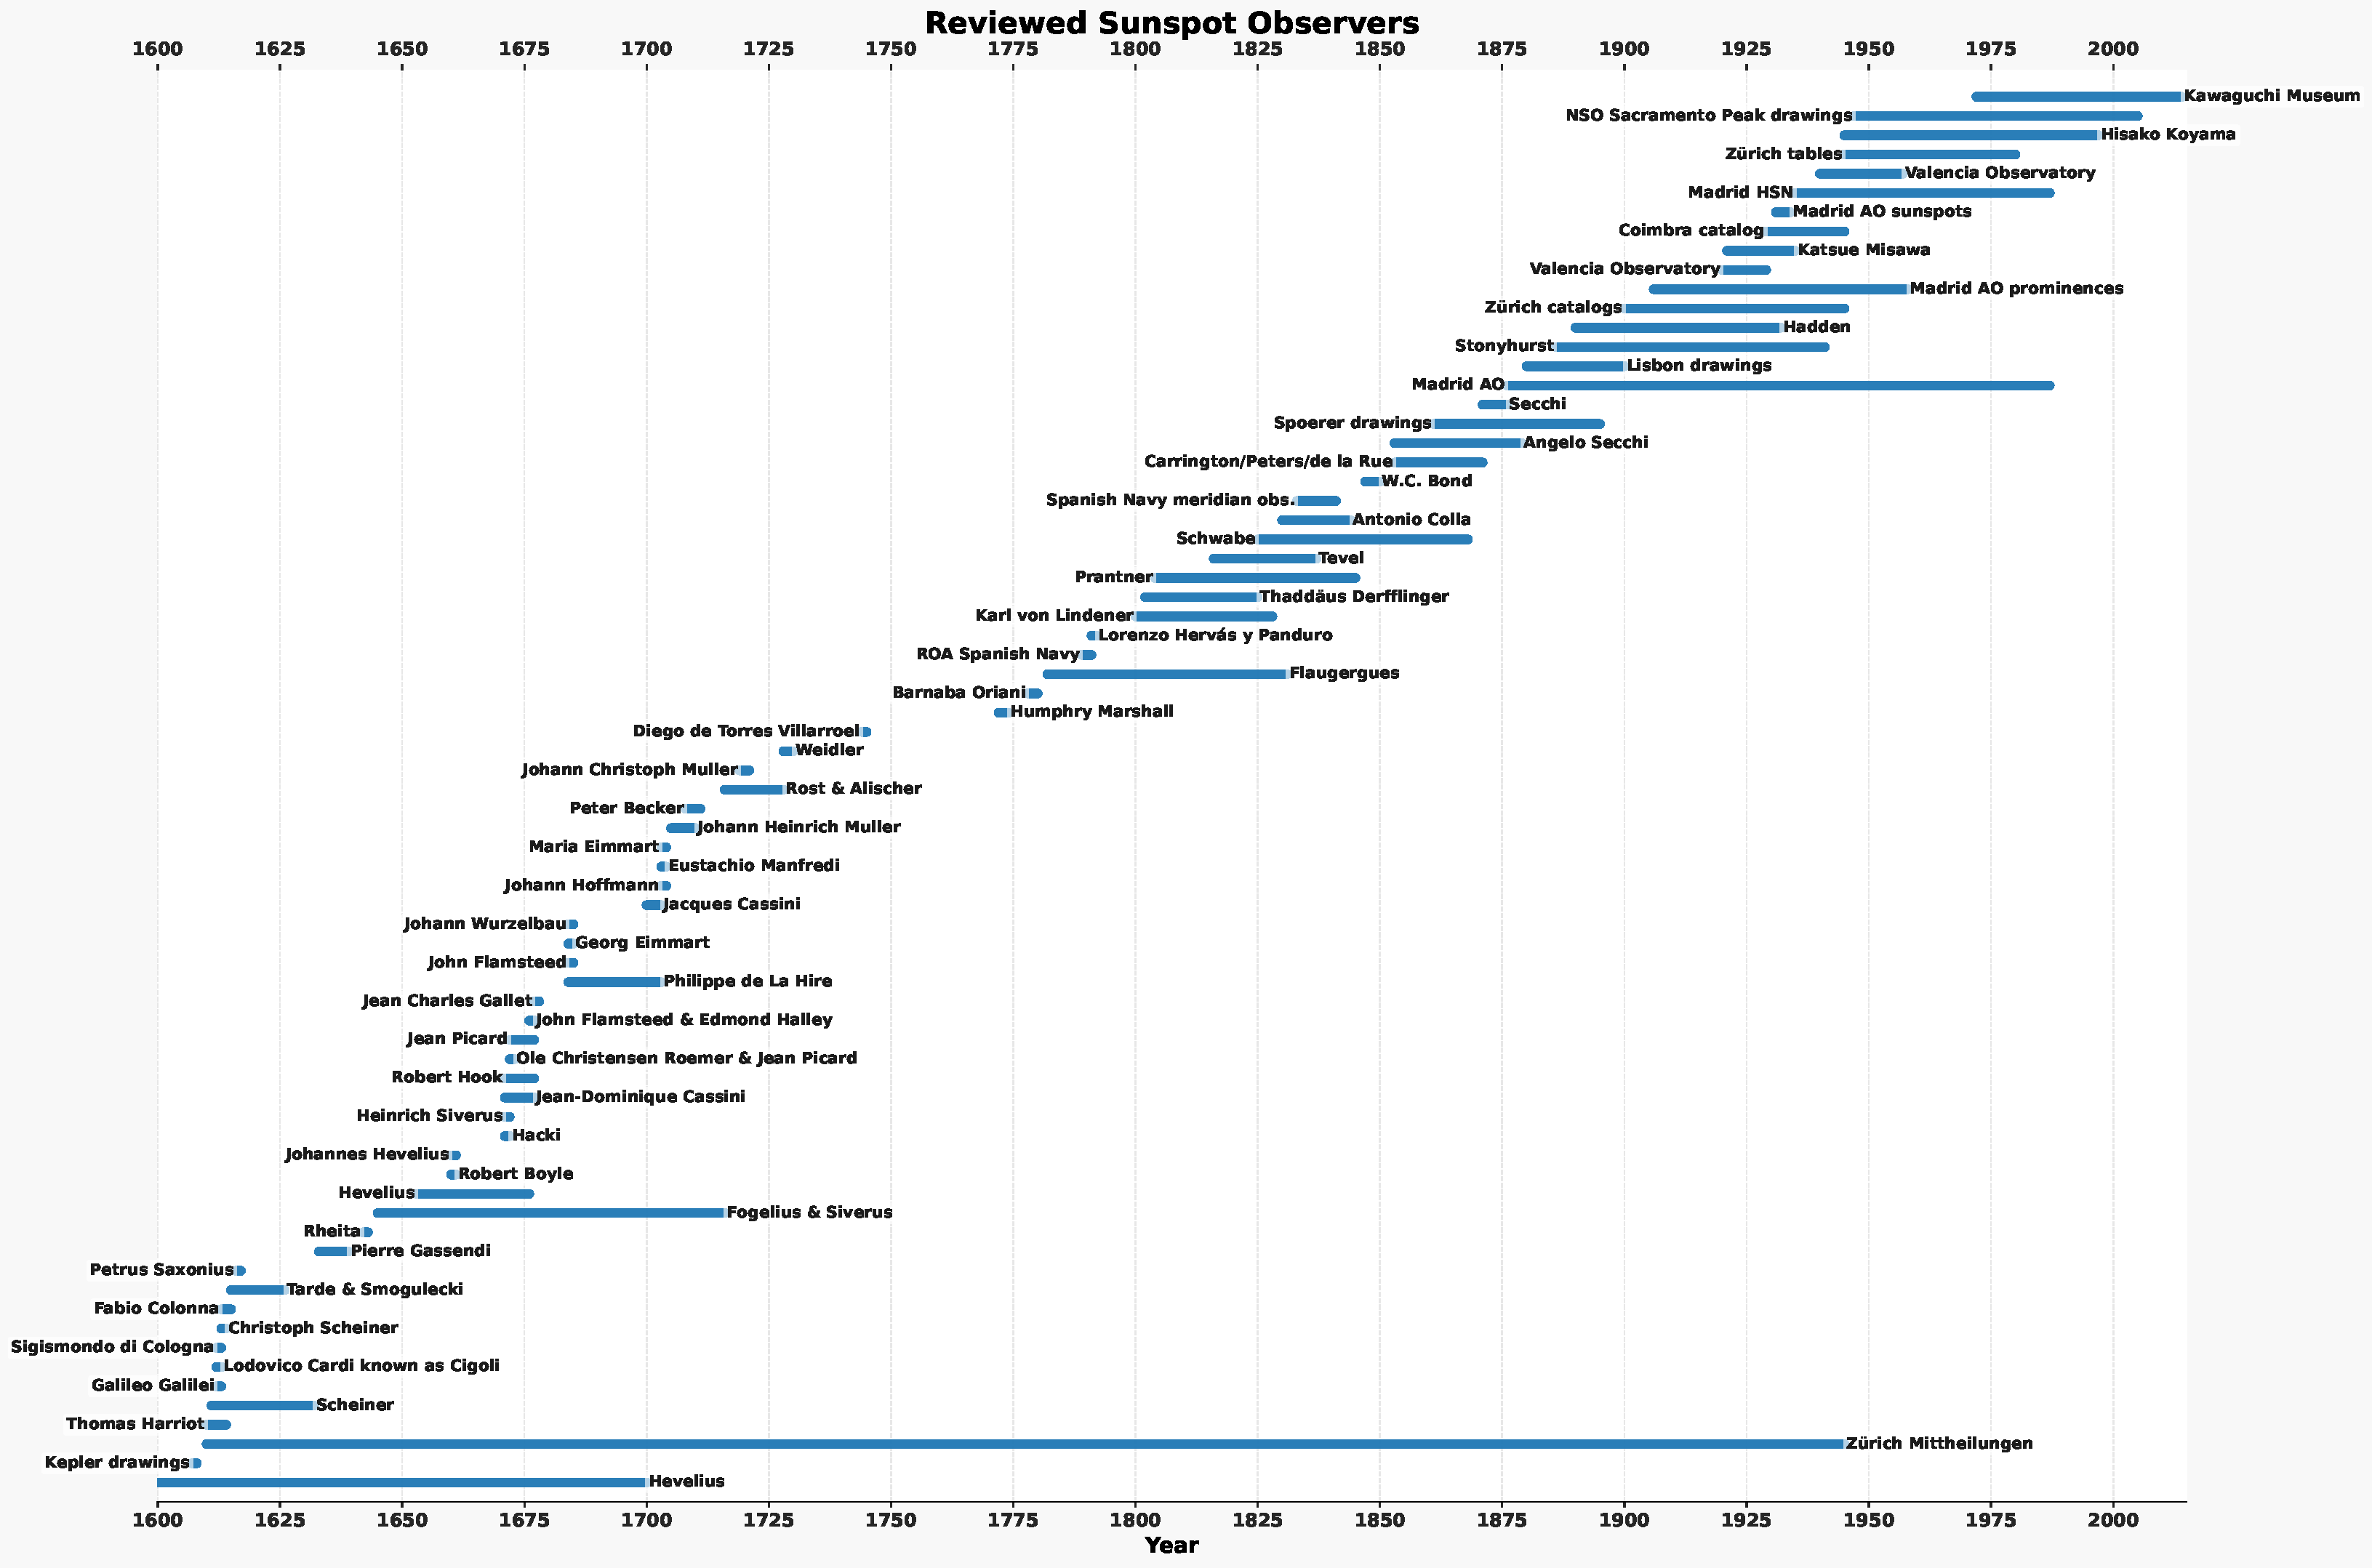
\includegraphics[width=\linewidth]{../figures/reviewed_sources_timeline_merged.pdf}
%
% A non-exhaustive set of early telescopic sunspot datasets recovered and published since 2010, showing their temporal coverage from the early 1600s to the modern era. Major contributions by Hayakawa, Arlt, Vaquero, Carrasco, and others have greatly expanded the number of available raw observations.
%
% \end{cardblock}
%
% % ------------------ PROGRESS HIGHLIGHTS ------------------
% \begin{cardblock}{Progress Highlights}
% \begin{itemize}
%   \item Citizen-science interface blueprint prepared for the upcoming transcription portal.
%   \item Zürich pipeline blends Transkribus extraction with manual review.
%   \item Gruithuisen workflow couples Kurrent experts with validation scripts.
%   \item Adams drawings cross-checked with \emph{Mittheilungen} spotless-day entries.
% \end{itemize}
% \end{cardblock}
%
% % ------------------ RAW \textrightarrow  SN V3.0 ------------------
% \begin{cardblock}{From Raw to SN V3.0}
% \begin{enumerate}
%   \item Curate daily counts with provenance-rich metadata (observer, instrument, weather).
%   \item Solve observer response functions to align group/spot scales across centuries.
%   \item Aggregate to monthly, yearly, and hemispheric indices with propagated uncertainties.
%   \item Benchmark against SN V2.0 and satellite-era proxies to validate drift corrections.
% \end{enumerate}
% \end{cardblock}
%
% % ------------------ CHALLENGES ------------------
% \begin{cardblock}{Challenges}
% \begin{itemize}
%   \item Deciphering \emph{Kurrent} manuscripts while retaining contextual notes.
%   \item Integrating heterogeneous formats (drawings, tabular ledgers, marginalia).
%   \item Quantifying observer bias and spotless-day reporting habits.
%   \item Maintaining end-to-end provenance from scanned folios to final data products.
% \end{itemize}
% \end{cardblock}
%
% % ------------------ SPACE CLIMATE IMPACT ------------------
% \begin{cardblock}{Space Climate Impact}
%
% \begin{minipage}[t]{0.48\linewidth}
%   \callout{\color{AGUblue}Citizen Science}{Interactive portal mobilises volunteers to transcribe \emph{Kurrent} manuscripts and support STEM outreach.}
% \end{minipage}
% \hfill
% \begin{minipage}[t]{0.48\linewidth}
%   \callout{\color{AGUblue}Forecasting}{Bias-free SN V3.0 improves solar cycle prediction and operational space weather baselines.}
% \end{minipage}
%
% \vspace{0.25em}
%
% \begin{minipage}[t]{0.48\linewidth}
%   \callout{\color{AGUblue}Climate Links}{Validated historical forcing refines long-term climate models and Earth's energy budget.}
% \end{minipage}
% \hfill
% \begin{minipage}[t]{0.48\linewidth}
%   \callout{\color{AGUblue}Open Science}{FAIR releases with APIs and uncertainty bundles accelerate community reuse.}
% \end{minipage}
%
% \end{cardblock}
%
% % ------------------ QR CODE ------------------
% \begin{cardblock}{Poster QR Code}
% \centering
% 
\includegraphics[width=0.3\linewidth]{../docs/figures/qrcode_farsun-poster.png}
% \par\vspace{0.2em}
% \small For more information on FARSuN project, datasets, and a digital copy of this poster, scan the QR code.
% \end{cardblock}
%
% \vspace{-0.5em}
% \par}
%
% \end{column}
%
%
% \end{document}
